%% For submission and review of your manuscript please change the
%% command to \documentclass[manuscript, screen, review]{acmart}.
%%
%% When submitting camera ready or to TAPS, please change the command
%% to \documentclass[sigconf]{acmart} or whichever template is required
%% for your publication.
%%
%%


\newif\ifcomments\commentstrue
%\newif\ifcomments\commentsfalse

\newif\iflong\longfalse
%\newif\iflong\longtrue

\newif\iftwocolumns\twocolumnstrue
%\newif\iftwocolumns\twocolumnsfalse


\documentclass[sigplan,screen,review]{acmart}
%%
%% \BibTeX command to typeset BibTeX logo in the docs
\AtBeginDocument{%
  \providecommand\BibTeX{{%
    Bib\TeX}}}

%% Rights management information.  This information is sent to you
%% when you complete the rights form.  These commands have SAMPLE
%% values in them; it is your responsibility as an author to replace
%% the commands and values with those provided to you when you
%% complete the rights form.
\setcopyright{acmlicensed}
\copyrightyear{2018}
\acmYear{2018}
\acmDOI{XXXXXXX.XXXXXXX}
%% These commands are for a PROCEEDINGS abstract or paper.
\acmConference[Conference acronym 'XX]{Make sure to enter the correct
  conference title from your rights confirmation email}{June 03--05,
  2018}{Woodstock, NY}
%%
%%  Uncomment \acmBooktitle if the title of the proceedings is different
%%  from ``Proceedings of ...''!
%%
%%\acmBooktitle{Woodstock '18: ACM Symposium on Neural Gaze Detection,
%%  June 03--05, 2018, Woodstock, NY}
\acmISBN{978-1-4503-XXXX-X/2018/06}


%%
%% Submission ID.
%% Use this when submitting an article to a sponsored event. You'll
%% receive a unique submission ID from the organizers
%% of the event, and this ID should be used as the parameter to this command.
%%\acmSubmissionID{123-A56-BU3}


\usepackage{macros}
\usepackage{laetitia_macro}

\usepackage{thmtools} 
\usepackage{thm-restate}
\usepackage{wrapfig}


\begin{document}

\theoremstyle{acmdefinition}
\newtheorem{remark}[theorem]{Remark}
\newtheorem{fact}[theorem]{Fact}

\title{Realisability and Complementability of Multiparty Session Types}

%%
%% The "author" command and its associated commands are used to define
%% the authors and their affiliations.
%% Of note is the shared affiliation of the first two authors, and the
%% "authornote" and "authornotemark" commands
%% used to denote shared contribution to the research.

\author{Cinzia {Di Giusto}}
\email{cinzia.di-giusto@univ-cotedazur.fr}
\orcid{0000-0003-1563-6581}

\author{Etienne Lozes }
\email{etienne.lozes@univ-cotedazur.fr}
\orcid{0000-0001-8505-585X}

\author{Pascal Urso }
\email{pascal.urso@univ-cotedazur.fr}


\affiliation{
	\institution{Université Côte d’Azur, CNRS, I3S}
	\country{France}}
	

%%
%% By default, the full list of authors will be used in the page
%% headers. Often, this list is too long, and will overlap
%% other information printed in the page headers. This command allows
%% the author to define a more concise list
%% of authors' names for this purpose.
%\renewcommand{\shortauthors}{Trovato et al.}

%%
%% The abstract is a short summary of the work to be presented in the
%% article.
\begin{abstract}
	% !TEX root =  ../mainPPDP.tex
%!TEX spellcheck = en_GB


%TITLE: Realisability and Complementability of Multiparty Session Types 


%Multiparty session types (MPST) are a type-based approach for specifying message-passing distributed systems.
%MPST rely on the notion of global type specifying the global behaviour and local types which are the projections of the global behaviour onto each local participant. An essential property of global types is implementability, i.e., whether the composition of the local behaviours conforms to those specified by the global type. 
%MPST have been studied extensively but almost solely for peer-to-peer communications. 
%In this paper, we generalise the implementability problem to any communication model.
%First, we show that if a global type is implementable in an arbitrary communication model,
%then it is implementable in the synchronous model. Second, we show that if a global type is implementable in the synchronous model, then it is complementable, in the sense that there exists a global type that describes the complementary behaviour of the original global type.
%Third, we give an algorithm to decide whether a complementable global type, given with an explicit complement, is 
%implementable in a communication model. The algorithm is PSPACE in the size of the global type and its complement, when the communication model is fixed. Finally, we propose a complementation construction for global types with sender driven choice with a linear blowup in the size of the global type.


Multiparty session types (MPST) are a type-based approach for specifying message-passing distributed systems.
They rely on the notion of global type specifying the global behaviour and local types which are the projections of the global behaviour onto each local participant. An essential property of global types is realisability, i.e., whether the composition of the local behaviours conforms to those specified by the global type.
We explore how realisability of MPST relates to their complementability, i.e., whether there exists a global type that describes the complementary behaviour of the original global type.
First, we show that if a global type is realisable with p2p communications, then it is realisable with synchronous communications. Second, we show that if a global type is realisable in the synchronous model, then it is complementable, in the sense that there exists a global type that describes the complementary behaviour of the original global type.
Third, we give an algorithm to decide whether a complementable global type, given with an explicit complement, is 
realisable in p2p. The algorithm is PSPACE in the size of the global type and its complement. As a side contribution, we propose a complementation construction for global types with sender-driven choice with a linear blowup in the size of the global type.
\end{abstract}

%%
%% The code below is generated by the tool at http://dl.acm.org/ccs.cfm.
\begin{CCSXML}
<ccs2012>
<concept>
<concept_id>10003752.10003766.10003776</concept_id>
<concept_desc>Theory of computation~Regular languages</concept_desc>
<concept_significance>300</concept_significance>
</concept>
<concept>
<concept_id>10003752.10003753.10003761.10003764</concept_id>
<concept_desc>Theory of computation~Process calculi</concept_desc>
<concept_significance>500</concept_significance>
</concept>
<concept>
<concept_id>10003752.10003790.10011740</concept_id>
<concept_desc>Theory of computation~Type theory</concept_desc>
<concept_significance>500</concept_significance>
</concept>
<concept>
<concept_id>10003752.10010124.10010138.10010143</concept_id>
<concept_desc>Theory of computation~Program analysis</concept_desc>
<concept_significance>500</concept_significance>
</concept>
</ccs2012>
\end{CCSXML}

\ccsdesc[300]{Theory of computation~Regular languages}
\ccsdesc[500]{Theory of computation~Process calculi}
\ccsdesc[500]{Theory of computation~Type theory}
\ccsdesc[500]{Theory of computation~Program analysis}

%%
%% Keywords. The author(s) should pick words that accurately describe
%% the work being presented. Separate the keywords with commas.
\keywords{Multiparty session types, deadlock-freedom, synchronizability, message-sequence-charts}


\received{20 February 2007}
\received[revised]{12 March 2009}
\received[accepted]{5 June 2009}

\maketitle

\section{Introduction}
	% !TEX root =  ../mainPPDP.tex
%!TEX spellcheck = en_GB

The design of communication protocols for concurrent and distributed systems is a central concern in programming language research. 
Modern systems —- from microservices to IoT networks -— rely on structured sequences of message exchanges between multiple parties. 
In the family of behavioural types~\cite{DBLP:conf/concur/VasconcelosH93}, multiparty session types (MPST), as introduced by Honda et al.~\cite{HondaYC08,10.1145/2873052,DBLP:conf/icdcit/YoshidaG20}, have emerged as a powerful methodology to specify and verify such structured interactions. 
An MPST defines a global type describing the communication protocol as a whole, which can be projected into local types for each participant.% (as opposed to binary session types \cite{10.1007/3-540-57208-2_35,10.1007/3-540-58184-7_118,10.1007/BFb0053567} that only describe binary exchanges).

This type-based approach enables static verification of communication safety (no message type mismatches) and liveness properties (no deadlocks) by ensuring each party's code conformes to its local type. 
In essence, MPSTs allow protocol designers to treat communication patterns as first-class abstractions, yielding a rigorous framework for building correct distributed applications. 

In this work, we focus on the realisability problem, i.e., whether the local types projected from a global type can be recomposed into a concrete system that conforms to the intended global protocol\footnote{In classical MPST papers, this problem is also referred to as the implementability or projectability problem. We preferred to stick to realisability as a reference to the work by Alur et al. \cite{DBLP:journals/tcs/AlurEY05}.}. In classical MPST theory, protocols are often formulated under the sender-driven choice assumption: only one designated participant (the sender) decides between alternative message flow branches for all parties. 
While this assumption simplifies theoretical analysis, it proves too restrictive for many real-world protocols. 
Modern distributed applications typically involve multiple independent agents that can initiate interactions concurrently, requiring more flexible interaction patterns than a single centralised decision maker.
To illustrate the limitation of sender-driven choice, consider a simplified publish/subscribe scenario inspired by the MQTT (Message Queuing Telemetry Transport) protocol~\cite{mqtt311}.  Suppose we  have two client
\begin{wrapfigure}{r}{0.25\textwidth}
  \begin{center}
%\begin{figure}
    \begin{tikzpicture}[>=stealth, node distance=2cm, auto]
        % État initial
        \node[state, initial, initial text={}, initial distance=3mm, minimum size=1.5em] (s0) {\tiny$s_0$};
    
        % États pour publication c1 -> c2
        \node[state, minimum size=1.5em] (s1) [above right=2cm and 1cm of s0] {\tiny$s_1$};
        \node[state, minimum size=1.5em] (s2) [right=2cm of s0] {\tiny$s_2$};
    
        % Boucle de publication de c1
        \draw[->, bend left=40] (s0) to node[above,sloped]{\tiny$\gtlabel{c1}{b}{pub(m)}$}(s1);
        \draw[->, bend right=20] (s1) -- node[above,sloped] {\tiny$\gtlabel{b}{c2}{pub(m)}$} (s0);

        % Boucle de publication de c2
        \draw[->, bend left=20] (s0) to node[above,sloped]{\tiny$\gtlabel{c2}{b}{pub(m)}$}(s2);
        \draw[->, bend right=20] (s2) -- node[below,sloped]{\tiny$\gtlabel{b}{c1}{pub(m)}$} (s0);
    \end{tikzpicture}
    \caption{\label{fig:MQTT}MQTT protocol with two clients}
     \end{center}
\end{wrapfigure}
%\end{figure}
  processes (publisher/subscribers) $c_1$ and $c_2$ connected to a broker $b$. 
Both clients can independently publish messages to the broker, which in turn forwards each message to the other client. % (see Figure~\ref{fig:MQTT}). 
After the initial setup (e.g., subscriptions to topics not described here), either $c_1$ or $c_2$ may send a message at any time, without a predefined order. 
This pattern cannot be  captured by a sender-driven global type, as the choice of which client sends a message next is not controlled by any of the  participants.  In a sender-driven MPST, one would have to arbitrarily fix one client as the decision maker for the communication branch, which fails to reflect the  nature of the interaction.
%This example motivates the need to go beyond sender-driven protocols and to develop a theory of implementability for more general multiparty communications.

% MQTT 2-clients protocol global type

\subsubsection*{Contributions}In this work, we approach the realisability question from a language design perspective. We consider two  fundamental communication models for implementing MPST protocols: the asynchronous peer-to-peer ($\ppmodel$) model and the synchronous one.
In the $\ppmodel$ model, processes communicate via point-to-point asynchronous message passing over FIFO channels, which is the standard mode for distributed systems.
In the synchronous model, communications are rendezvous-based (handshakes where send and receive happen simultaneously), representing a globally synchronised message-passing semantics. 
These two models are widely considered as canonical extremes in analysing distributed protocols. 
A large amount of our approach generalises to even more communication models, but a full generalisation is beyond the scope of this paper,
and we only reason on general communication models for purpose of defining a notion of realisability that is parametric in the communication model (see Definition~\ref{def:realisability}).

In this work, we also investigate for the first time the question of the complementability of global types, 
i.e., whether a global type can be complemented by another global type that describes all possible complementary behaviours.
This notion may seem at first sight rather theoretical and unrelated to realisability, but our work reveals deep relations between
these two notions.

Our main contribution is to show that realisable global types form a subclass of the complementable ones.
More in details, we establish the following results:

\begin{itemize}
\item Every global type realisable in the synchronous communication model is complementable (Theorem~\ref{thm:realisable-complementable}), and the complementation is
effective (based on projection and NFA complementation)
\item Realisability is decidable in PSPACE for complementable global types provided an explicit complement is also given as input,
both in the synchronous communication model (Theorem~\ref{thm:decidability-of-implementability-in-synch}) and in the peer-to-peer model 
(Theorem~\ref{thm:decidability-of-implementability-in-p2p}), the latter result being based on recent results on RSC systems~\cite{germerie-phd}.
\item On the way, we show that if a global type is realisable in the peer-to-peer model, then it is also realisable in the synchronous one (Theorem~\ref{thm:pp-realizability-implies-synch-realizability}), which is not obvious, as 
deadlock-freedom is not a property that is monotonic in the communication model (a more permissive communication model may both hide some deadlocks and trigger new ones)
\item We collect several interesting observations about the question of the complementability of global types: not all global types are complementable (Example~\ref{ex:non-complementable-gt}),
but global types with at most three participants are complementable (Corollary~\ref{coro:3-participants-complementable}), 
as well as global types with sender-driven choices (Theorem~\ref{thm:sender-driven-choice-complementation}). For the latter, we provide
a complementation procedure with a linear blowup in the size of the global type.
\end{itemize}


% The communication models mentioned before form a hierarchy from relaxed to more constrained communication models, either in terms
% of executions~\cite{DBLP:conf/fm/ChevrouH0Q19}, or in terms of message sequence 
% charts~\cite{DBLP:journals/pacmpl/GiustoFLL23}.
% Several interesting properties turns out to be monotonic in the communication model in the following sense: if a property is satisfied in a communication model, then it is preserved for more relaxed (resp. more constrained) ones. 
% This  is true, for instance, when checking for reachability of a configuration,
% for unspecified receptions (the first message in a queue cannot be received by its
% destination process), orphan messages (i.e., messages sent by a peer but never received), etc.
% Unfortunately, implementability is not monotonic.
% To better understand this, take the following  two examples. First, consider an example of a global type (in standard MPST syntax) that is implementable in the peer-to-peer model but not in the mailbox one:  $$\gt_1 = \gtlabel{p}{q}{\msg_1} . \gtlabel{r}{q}{\msg_2} . \mathsf{end}.$$
%  This global type is implementable in the peer-to-peer model, 
% because the projection $p\parallel q \parallel r= !\msg_1 \parallel ?\msg_1.?\msg_2\parallel !\msg_2$ is deadlock-free and session conformant. However, this global type is not implementable in the mailbox model, where all incoming messages of process $q$ are stored in a unique FIFO queue,
% because $\msg_2$ could be sent and hence stored in the queue before $\msg_1$  and cause a deadlock.
% Second, consider this example where the converse happens: 
% %%
% $$ 
% \begin{array}{lll}
% \gt_2 & = & \gtlabel{p}{q}{\msg_1} . \textcolor{red}{\gtlabel{p}{r}{\msg_2}} . \gtlabel{p}{q}{\msg_3} 
%         . \textcolor{blue}{\gtlabel{q}{r}{\msg_4}} . \mathsf{end} 
% \\
% & + & \gtlabel{p}{q}{\msg_1'} . \textcolor{blue}{\gtlabel{q}{r}{\msg_4}} . \gtlabel{q}{p}{\msg_3'} 
%         . \textcolor{red}{\gtlabel{p}{r}{\msg_2}} . \mathsf{end}  
% \end{array}
% $$
% %%
% This global type $\gt_2$ is depicted in Figure~\ref{fig:gt2}, it features two possible
% scenarios, starting either with $\msg_1$ or $\msg_1'$, (that  are depicted on the left). 
% It is not implementable in the peer-to-peer model, because the projection 
% $p\parallel q \parallel r$ also admits the interaction where  $p$ and $q$ follow the first scenario, but $r$ follows the second scenario, resulting in a non synchronisable interaction (also depicted in Figure~\ref{fig:gt2}). However, this global type is implementable in the mailbox model, because the messages sent to $r$ are stored in a unique FIFO queue, and their order in the queue, is sufficient for  $r$ to  not confuse the two scenarios.
% \begin{figure}
%     \begin{tikzpicture}[scale=0.7]
%         \begin{scope}
%             \newproc{0}{p}{-2.7};
%             \newproc{2}{q}{-2.7};
%             \newproc{4}{r}{-2.7};

%             \newmsgm{0}{2}{-0.3}{-0.3}{1}{0.5}{black};
%             \newmsgm{0}{4}{-1.0}{-1.0}{2}{0.25}{red};
%             \newmsgm{0}{2}{-1.7}{-1.7}{3}{0.5}{black};
%             \newmsgm{2}{4}{-2.4}{-2.4}{4}{0.5}{blue};
%         \end{scope}

%         \begin{scope}[xshift=7cm]
%             \newproc{0}{p}{-2.7};
%             \newproc{2}{q}{-2.7};
%             \newproc{4}{r}{-2.7};

%             \newmsgm{0}{2}{-0.3}{-0.3}{1'}{0.5}{black};
%             \newmsgm{2}{4}{-1.0}{-1.0}{4}{0.5}{blue};
%             \newmsgm{2}{0}{-1.7}{-1.7}{3'}{0.5}{black};
%             \newmsgm{0}{4}{-2.4}{-2.4}{2}{0.25}{red};
%         \end{scope}

%         \begin{scope}[xshift=14cm]
%             \newproc{0}{p}{-2.7};
%             \newproc{2}{q}{-2.7};
%             \newproc{4}{r}{-2.7};

%             \newmsgm{0}{2}{-0.3}{-0.3}{1}{0.5}{black};
%             \newmsgm{0}{4}{-1.0}{-2.4}{2}{0.25}{red};
%             \draw[>=latex,->] (0,-1.45) -- node [below, pos = 0.25] {$\msg_{3}$} (2,-1.45);
%             \newmsgm{2}{4}{-1.95}{-1.95}{4}{0.5}{blue};
%         \end{scope}

%     \end{tikzpicture}
%     \caption{The two interactions specified by $\gt_2$, and another unspecified interaction that happens in the projected system in the p2p semantics}\label{fig:gt2}
% \end{figure}
% %%


% These two examples show that "implentability is not monotonic",
% and suggest that every new communication model should prompt the development of a new ad hoc theory of implementable global types, with its own syntactic conditions.



%\cinzia{add precision to contributions and fix Outline}
\subsubsection*{Outline.} The paper is organised as follows: Section~\ref{sec:preliminaries} introduces the necessary background on executions, Message Sequence Charts, communication models and communicating finite state machines. 
MPST and realisability are introduced in Section~\ref{sec:global_types}. Then Section \ref{sec:complementability} discusses the notions of effectively complementable and give examples of known global types that follow in this class. Finally Section~\ref{sec:decidability}  shows  our results on the reduction of realisability to the synchronous communication model based on the notion of effectively complementable global types.  
Section \ref{sec:concl} concludes with some final remarks and discusses related works.
%An appendix containing proofs and additional material has been included for the reviewer’s convenience.





	\section{Preliminaries}\label{sec:preliminaries}
	% !TEX root =  ../mainPPDP.tex
%!TEX spellcheck = en_GB


%In this section we introduce some notation to talk about communicating automata, executions and message sequence charts.

We assume a finite set of \emph{processes} $\Procs=\{p,q,\ldots\}$ and a finite set of messages (labels) 
$\Msg=\{\msg,\ldots\}$.
We consider two kinds of actions:  \emph{send actions} that are  of the form 
$\send{p}{q}{\msg}$ and are executed by  process $p$  sending message  $\msg$ to  $q$;
 \emph{receive actions} that are of the form $\recv{p}{q}{\msg}$ and are executed by  $q$ receiving  $\msg$ from  $p$.
We write $\Act$ for the finite set $\Procs\times\Procs\times\{!,?\}\times\Msg$ of all actions, and $\Actp$ for the set of actions 
that can be executed by $p$ (i.e., $\send{p}{q}{\msg}$ or $\recv{q}{p}{\msg}$). 
We omit processes when they are clear from the context and simply write $!\msg$ or $?\msg$ for a send or receive action, respectively.

An \emph{event} $\event$ of a sequence of actions $w\in \Act^*$, is an index $i$ in $\{1,\ldots,\length{w}\}$;
$i$ is a send (resp. receive) event of $w$ if $w[i]$ is a send (resp. receive) action.
We write $\sendeventsof{w}$ (resp. $\receiveeventsof{w}$) for the set of send (resp. receive) events 
of $w$ and $\eventsof{w}=\sendeventsof{w}\cup\receiveeventsof{w}$ for the set of all events of $w$.
When all events are labeled with distinct actions, we identify an event with its action.



\subsubsection*{Executions.}
An execution is a well defined sequence of actions $e\in\Act^*$, where 
a receive action is always preceded by a unique corresponding send action.


\begin{definition}[Execution]
	An \emph{execution} over $\Procs$ and $\Msg$ is a sequence of actions $e\in\Act^*$  
	where an injective function from receive events to send events $\source_{e}:\receiveeventsof{w}\to\sendeventsof{w}$ 
	can be defined such that for each receive event $i$ labeled with $\recv{p}{q}{\msg}$,
	 $\source_{e}(i)$ is labeled with $\send{p}{q}{\msg}$, and  $\source_{e}(i)<i$.
\end{definition}


%For two events $i,j\in\eventsof{e}$, we write $i\hbstrictof{e}{} j$ if $i<j$ (order on natural numbers).
%When all send actions of a sequence of actions $w$ are distinct, there is at most one execution 
%$\execution$ such that $w$ is the sequence of actions of $\execution$, and we often identify $w$ with $\execution$
%and let $\source$ be implicit. 

%An execution $\w_1$ is a \emph{prefix} of $w_2$ if $w_1$ is a prefix of $w_2$ and 
%$\source_1$ is the restriction of $\source_2$ to $\receiveeventsof{w_1}$.
For a set of executions $\mathcal{E}$, we write $\prefixclosureof{\mathcal{E}}$ 
for the set of all prefixes of the executions in $\mathcal{E}$. 
We say that an execution $e_2$ is a \emph{completion} of an execution $e_1$
if $e_1$ is a prefix of $e_2$. 
A \emph{concatenation} $e_1\cdot w$ of an execution
$e_1$ and a sequence of actions $w$ is the execution $e_2 = e_1\cdot w_2$ where 
$e_2$ is a completion of $e_1$ (note that $w$ is not an execution, since it may contain receive events
which sources are in $e_1$).  
The \emph{projection} $\projofon{e}{p}$ of an execution $e$ on a process $p$ 
is the subsequence of actions in $\Actp$.  
A send event $s$ is \emph{matched} if there is a receive event $r$ such that $s=\source(r)$.
An execution $e$ is \emph{orphan-free} if $\source$ is surjective over the send events of $e$, i.e.,
all send events are matched.

\subsubsection*{Communication Models.}
In this paper, we consider   two communication models: 
peer-to-peer ($\ppmodel$) and  synchronous ($\synchmodel$). 
However, as commented  in the conclusions,  this work is part of a bigger more general project and a large amount of the results of the paper can be extended to "any" communication model, or 
only require  few assumptions.  In this perspective, we  introduce a general definition of a communication model here
and discuss on specific results on how they can be extended to the general case.
\begin{definition}[Communication model]
	\label{def:communication-model}
	A \emph{communication model} $\acommunicationmodel$ is a set 
	$\executionsofmodel{\acommunicationmodel}$ of executions.
\end{definition}
% It is \emph{prefix-closed} if 
% $\executionsofmodel{\acommunicationmodel}$ is prefix-closed, i.e., for all
% $e,e'\in\executionsofmodel{\acommunicationmodel}$, if $e\prefixorder e'$, then $e\in\executionsofmodel{\acommunicationmodel}$.

In the  synchronous communication model $\synchmodel$, message exchanges can be thought as rendez-vous synchronisations.
In other words, an execution $e$ belongs to $\executionsofmodel{\synchmodel}$ if
all send events are immediately followed by their corresponding receive events.
\begin{definition}[Synchronous communication model]
	An execution $\execution=(w,\source) \in \executionsofmodel{\synchmodel}$ if
	for all send event $s\in\sendeventsof{e}$, $s+1$ is a receive event of $e$ and $\source(s+1)=s$.
\end{definition}

In the peer-to-peer communication model $\ppmodel$, messages sent by a process $p$ to $q$ transit over a FIFO channel
that is specific to the pair $(p,q)$: if $p$ sends first $m_1$ then $m_2$ to $q$, 
then $m_2$ cannot overtake $m_1$ in the FIFO channel. In particular:
\begin{itemize}
	\item if $m_1$ is not received, then $m_2$ is not received either;
	\item if both are received, then $m_1$ is received before $m_2$.
\end{itemize}
      
\begin{definition}[$\ppmodel$ communication model]\label{def:queue-based-communication-model}
	$\executionsofmodel{\ppmodel}$  is
	the set of executions $e$ such that for any two send events $s_1=\send{p}{q}{\msg_1}$ and 
	$s_2=\send{p}{q}{\msg_2}$ in $\sendeventsof{e}$, 
	with $s_1 < s_2$,
	one of the two holds:
	\begin{itemize}
		\item $s_2$ is unmatched, or
		\item there exists $r_1,r_2$ such that $r_1<r_2$, $\source(r_1)=s_1$, and $\source(r_2)=s_2$.
	\end{itemize}
\end{definition}

Note that, $\executionsofmodel{\synchmodel}\subset\executionsofmodel{\ppmodel}$.
Moreover, if $e$ is an execution in $\ppmodel$, then  $\source_e$ is defined as follows:
the source of the $i$-th receive event of $q$ from $p$ is the $i$-th send event of $p$ to $q$.
If $e$ is an execution in $\synchmodel$, then $\source_e$ is defined as follows: 
for all receive event $i$, $\source_{e}(i)=i-1$.


\subsubsection*{Message Sequence Charts.}
While executions correspond to a total order view of the events occurring in a 
system, message sequence charts (MSC) adopt a distributed, a partial order view on the events.
For a tuple $\msc=(w_p)_{p\in\Procs}$, each $w_p\in\Actsp$ 
is a sequence of actions representing  the ones executed by process $p$ according to some total, locally observable, order.
We write $\eventsof{\msc}$  for the set $\{(p,i) \mid p \in \Procs \text{ and } 0 \leq i < \length{w_p}\}$.
The label $\actionof{\event}$ of the event $\event=(p,i)$ is the action $w_p[i]$. The event $\event$
is a send (resp. receive) event if it is labeled with a send (resp. receive) action.
We write $\sendeventsof{\msc}$ (resp. $\receiveeventsof{\msc}$) for the set of send (resp. receive) events of $\msc$; we also write $\messageof{\event}$ for the message sent or received at event $\event$, and 
$\processof{\event}$ for the process executing $\event$. Finally, we write 
$\verticalorderstrict{\event_1}{\event_2}$ if there is a process $p$ and $i<j$ such that
$\event_1=(p,i)$ and $\event_2=(p,j)$.
%\pascal{Notations $\sendevents{\msc}$,  $\messageof{e}$, $\receiveevents{\msc}$ and $\processof{e}$ are used once in the paper. Should we keep them?}

\begin{definition}[MSC]\label{def:msc}
	An {MSC} over $\Procs$ and $\Msg$ is a tuple $\msc = \big((w_p)_{p\in\Procs},\source\big)$
    where
    \begin{enumerate}
        \item for each process $p$, $w_p\in\Actsp$ is a finite sequence of actions;
        \item $\source: \receiveeventsof{\msc} \to \sendeventsof{\msc}$ is 
            an injective function from receive events to send events such that
			for all receive event $\event$ labeled with $\recv{p}{q}{\msg}$,
            $\source(\event)$ is labeled with $\send{p}{q}{\msg}$.
    \end{enumerate}
\end{definition}

\begin{figure}[t]
		\captionsetup[subfigure]{justification=centering}
	% \centering
	\begin{subfigure}[t]{0.22\textwidth}\centering

		\begin{tikzpicture}[scale=0.7, every node/.style={transform shape}]
			\newproc{0}{p}{-2.2};
			\newproc{2}{q}{-2.2};

			\newmsgm{0}{2}{-1.7}{-0.5}{1}{0.25}{black};
			\newmsgm{2}{0}{-1.7}{-0.5}{2}{0.25}{black};

			\end{tikzpicture}
		\caption{non-linearisable MSC}	\label{fig:raw_msc_ex}

		\end{subfigure}
%        \begin{subfigure}[t]{0.24\textwidth}\centering
%
%            \begin{tikzpicture}[scale=0.7, every node/.style={transform shape}]
%                \newproc{0}{p}{-2.2};
%                \newproc{2}{q}{-2.2};
%    
%                \newmsgm{0}{2}{-0.5}{-1.5}{1}{0.1}{black};
%                \newmsgm{0}{2}{-1}{-1}{2}{0.8}{black};
%    
%                \end{tikzpicture}
%            \caption{$\bagmodel$, and $\erlangmodel$ if $m_1\neq m_2$}	\label{fig:bag_ex}
%    
%            \end{subfigure}
        % \centering
	\begin{subfigure}[t]{0.22\textwidth}\centering
		\begin{tikzpicture}[scale=0.7, every node/.style={transform shape}]
			\newproc{0}{p}{-2.2};
			\newproc{1}{q}{-2.2};
			\newproc{2}{r}{-2.2};

			\newmsgm{0}{1}{-0.3}{-2}{1}{0.15}{black};
			\newmsgm{0}{2}{-0.9}{-0.9}{2}{0.75}{black};
			\newmsgm{2}{1}{-1.5}{-1.5}{3}{0.5}{black};
			% \newmsgm{2}{1}{-2}{-2}{4}{0.5}{black};

			% \newflechevert{Purple}{0}{-0.3}{-0.9};
			% \newflechehor{Purple}{-0.9}{0}{2};
			% \newflechevert{Purple}{2}{-0.9}{-1.5};
		\end{tikzpicture}
		\caption{$\ppmodel$} \label{fig:pp_ex}
	\end{subfigure}
%	\begin{subfigure}[t]{0.24\textwidth}\centering
%		\begin{tikzpicture}[scale=0.7, every node/.style={transform shape}]
%			\newproc{0}{p}{-2.2};
%			\newproc{1}{q}{-2.2};
%			\newproc{2}{r}{-2.2};
%			\newproc{3}{s}{-2.2};
%	
%			\newmsgm{0}{3}{-0.6}{-0.6}{2}{0.8}{black};
%			\newmsgm{2}{3}{-1.1}{-1.1}{3}{0.5}{black};
%			\newmsgm{2}{1}{-1.5}{-1.5}{4}{0.5}{black};
%			\newmsgm{0}{1}{-0.3}{-2}{1}{0.5}{black};
%		\end{tikzpicture}
%		\caption{$\causalmodel$} \label{fig:causal_ex}
%	\end{subfigure}
	% \hfill
%\begin{subfigure}[t]{0.24\textwidth}\centering
%	\begin{tikzpicture}[scale=0.7, every node/.style={transform shape}]
%		\newproc{0}{p}{-2.2};
%		\newproc{1}{q}{-2.2};
%		\newproc{2}{r}{-2.2};
%		\newproc{3}{s}{-2.2};
%
%		\newmsgm{3}{0}{-0.6}{-0.6}{2}{0.2}{black};
%		\newmsgm{3}{2}{-1.1}{-1.1}{3}{0.5}{black};
%		\newmsgm{2}{1}{-1.5}{-1.5}{4}{0.5}{black};
%		\newmsgm{0}{1}{-0.3}{-2}{1}{0.5}{black};
%	\end{tikzpicture}
%			\caption{$\mbmodel$} \label{fig:mb_ex}
%\end{subfigure}
%\begin{subfigure}[t]{0.24\textwidth}\centering
%	\begin{tikzpicture}[scale=0.7, every node/.style={transform shape}]
%		\newproc{0}{p}{-2.2};
%		\newproc{1}{q}{-2.2};
%		\newproc{2}{r}{-2.2};
%
%		\newmsgm{0}{1}{-0.3}{-1.5}{1}{0.15}{black};
%		\newmsgm{1}{0}{-0.9}{-0.9}{2}{0.25}{black};
%		\newmsgm{1}{2}{-2}{-2}{3}{0.5}{black};
%		% \newmsgm{2}{1}{-2}{-2}{4}{0.5}{black};
%	\end{tikzpicture}
%		\caption{$\busmodel$} \label{fig:bus_ex}
%\end{subfigure}
\begin{subfigure}[t]{0.22\textwidth}\centering
	\begin{center}
		\begin{tikzpicture}[scale=0.7, every node/.style={transform shape}]
			\newproc{0}{p}{-2.2};
			\newproc{1}{q}{-2.2};
			\newproc{2}{r}{-2.2};
			\newproc{3}{s}{-2.2};

			\newmsgm{0}{1}{-0.5}{-0.5}{1}{0.5}{black};
			\newmsgm{2}{3}{-0.5}{-0.5}{2}{0.5}{black};
			\newmsgm{1}{2}{-1}{-1}{3}{0.5}{black};

		\end{tikzpicture}
		\caption{$\synchmodel$}
		\label{fig:rsc_ex}
	\end{center}
\end{subfigure}
\begin{subfigure}[t]{0.24\textwidth}\centering
	\begin{tikzpicture}[scale=0.7, every node/.style={transform shape}]
		\newproc{0}{p}{-2.2};
		\newproc{2}{q}{-2.2};

		\newmsgum{0}{2}{-0.8}{1}{0.2}{black};
		\newmsgm{0}{2}{-1.6}{-1.6}{2}{0.2}{black};

		\end{tikzpicture}
	\caption{MSC with an orphan message}	\label{fig:orphan_ex}
\end{subfigure}
		\caption{Examples of MSCs. The sender of a message is at the origin of the arrow and the receiver at the destination. Unmatched send events are depicted with dashed arrows.}\label{fig:exmscs}
\end{figure}

For an execution $\execution$,  $\mscof{\execution}$ is the MSC 
$\big((w_p)_{p\in\Procs},\source\big)$ where $w_p$ is the subsequence of $\execution$ restricted to the actions of $p$,
and $\source$ is the lifting of $\source_{\execution}$ to the events of $(w_p)_{p\in\Procs}$.


\begin{example}
    \label{ex:msc}
     MSC $\msc$ in Fig.~\ref{fig:raw_msc_ex} is an MSC over $\Procs=\{p,q\}$ and $\Msg=\{\msg_1,\msg_2\}$
    with $\msc=\large((w_p,w_q),\source\large)$, $w_p = ?\msg_2!\msg_1$, $w_q = ?\msg_1!\msg_2$, $\source((p,0)) = (q,1)$,
    and $\source((q,0)) = (p,1)$. Note that there is no execution $\execution$ such that 
	$\msc=\mscof{\execution}$ as all receptions precede the corresponding sends. On the other hand, the MSC
	in Fig.~\ref{fig:pp_ex} is $\mscof{\execution}$ for the execution $\execution$
	$=\large(!\msg_1!\msg_2?\msg_2!\msg_3?\msg_3?\msg_1,\source\large)$ where 
	$\source(3) = 2$, $\source(5) = 2$ and $\source(6) = 4$. It is the only execution that induces this MSC, but 
	in general there might exist several executions inducing the same MSC.
\end{example}

For a set of processes $\Procs$, 
an MSC $M=\big((w_p)_{p\in\Procs},\source\big)$ is the \emph{prefix} 
of another MSC $M'=\big((w'_p)_{p\in\Procs},\source'\big)$, in short $M \prefixorder M'$,
if for all $p\in\Procs$, $w_p$ is a prefix of $w'_p$ and $\source'(e)=\source(e)$ for all receive events $e$ of $M$.
The \emph{concatenation} of MSCs $M_1$ and $M_2$ is the MSC  $M_1\cdot M_2$ 
obtained by gluing "vertically"  $M_1$ before $M_2$:
formally, if $M_1=((w_p^1)_{p\in\Procs},\source_1)$ and $M_2=((w_p^2)_{p\in\Procs},\source_2)$, 
then $M_1\cdot M_2=((w_p)_{p\in\Procs},\source)$ where
%\begin{inparaenum}[(i)]
 %   \item 
    for all $p$, $w_p=w_p^1\cdot w_p^2$, and
 %   \item 
    $\source$ is defined by $\source(e) = \source_i(e)$ for all receive events $e$ of $M_i$ ($i=1,2$).
%\end{inparaenum}

\subsubsection*{Happens-before relation and linearisations}
%\etienne{TODO cette section et ailleurs: relire en faisant attention à la convention de notation entre ordres partiels $\prec$ et totaux $<$}
In a given MSC $M$,
an event $\event$ happens before  
another event $\event'$, if 
(i) $\event$ and $\event'$ are events
of a same process $p$ and happen in that order on 
the time line of $p$,
or (ii) $\event$ is send event matched by $\event'$,
or (iii) a sequence of such situations defines
a path from $\event$ to $\event'$.

\begin{definition}[Happens-before relation]
Let $M$ be an MSC. The happens-before relation over $M$
is the binary relation $\happensbeforestrict$ defined as 
the least transitive relation over $\eventsof{\msc}$ such that:
\begin{itemize}
   \item 
   for all 
   $p,i,j$, if $i<j$, then $(p,i)\happensbeforestrict (p,j)$, and
   \item 
   for all receive events $\event$, $\source(\event) \happensbeforestrict \event$.
\end{itemize}
\end{definition}

\begin{definition}[Linearisation]
	\label{def:linearisation}
	A \emph{linearisation} of an MSC $\msc$ is a
total order $\alinearisation$ on $\eventsof{\msc}$
	that refines $\happensbeforestrict$:  for all events $\event,\event'$, 
	if $\event\happensbeforestrict \event'$, then $\event\alinearisation \event'$. 
\end{definition}
We write $\linearisationsof{\msc}{}$ for the set of all linearisations of $\msc$.
We often identify a linearisation
with the execution it induces. 

\begin{example}
	\label{ex:linearisation}
	Let $\msc$ be the MSC in Fig.~\ref{fig:rsc_ex}. 
	Then $!m_1$ happens before $?m_1$, which
	happens before $!m_3$, and both $!m_3$ and $!m_2$
	happen before $?m_3$.
	Moreover, $\happensbeforestrict$ is a partial order, 
	and 
	$!m_1!m_2?m_1!m_3?m_3?m_2 \in \linearisationsof{\msc_c}{}$.
	On the other hand, consider the MSC $M$ in 
	in Fig.~\ref{fig:raw_msc_ex}; then
	$\happensbeforestrictof{\msc'}$ is not a partial order, because
	$?m_2\happensbeforestrictof{\msc'}!m_1\happensbeforestrictof{\msc'}?m_1\happensbeforestrictof{\msc'}!m_2\happensbeforestrictof{\msc'}?m_2$,
	therefore $\linearisationsof{\msc'}{}=\emptyset$.
\end{example}


Given an MSC $\msc$, we write 
$\linearisationsof{\msc}{\acommunicationmodel}$
to denote 
$\linearisationsof{\msc}{}\cap\executionsofmodel{\acommunicationmodel}$; 
the executions of $\linearisationsof{\msc}{\acommunicationmodel}$
are called the linearisations of $\msc$ 
in the communication model $\acommunicationmodel$. 	

\begin{definition}[$\acommunicationmodel$-linearisable MSC]
	\label{def:linearisable-msc}
	An MSC $\msc$ is \emph{linearisable} in a communication model $\acommunicationmodel$ if 
	$\linearisationsof{\msc}{\acommunicationmodel}\neq\emptyset$.
	We write $\mscsetofmodel{\acommunicationmodel}$ for the set of all MSCs linearisable in $\acommunicationmodel$.
\end{definition}

\begin{example}
	\label{ex:msc-linearisable}
	The MSC $M_b$ in Fig.~\ref{fig:pp_ex} is linearisable in $\ppmodel$,
	with $\linearisationsof{M_b}{\ppmodel}=
%	$ 
%	$$
		\{!m_1!m_2?m_2!m_3?m_3?m_1\}
		$.
%	$$
	However, $M_b$ is not linearisable in $\synchmodel$.
	Finally the MSC $M_c$ in Fig.~\ref{fig:rsc_ex} is linearisable in $\synchmodel$ with
	$\linearisationsof{M_c}{\synchmodel}=$
	$$
	\{~!m_1?m_1!m_2?m_2!m_3?m_3~,~
	   !m_2?m_2!m_1?m_1!m_3?m_3~\}
	$$
\end{example}

Finally, we introduce a property that will be helpful in the next paragraph 
for
giving an alternative characterisation of deadlock-freedom of a system of communicating finite state machines.

\begin{definition}[Causally-closed communication model]\label{def:causally-closed-communication-model}
	A communication model $\acommunicationmodel$ is \emph{causally-closed} if for all MSCs $M$,
	$\linearisationsof{\msc}{\acommunicationmodel}\neq\emptyset$ implies that
	$\linearisationsof{\msc}{\acommunicationmodel}=\linearisationsof{\msc}{}$.
\end{definition}


  
  % !TEX root =  ../mainPPDP.tex
%!TEX spellcheck = en_GB
Observe that not all communication models are causally closed. It is the case for $\ppmodel$,  but it is immediate  to see that the property is not valid  for $\synchmodel$. Take for instance  MSC $M$ in Fig.~\ref{fig:rsc_ex},  its linearisation 
$!m_1!m_2?m_1?m_2!m_3?m_3$ 
  does not belong to $\linearisationsof{M_c}{\synchmodel}$.  To show that $\ppmodel$ is causally closed, 
notice that $<$ can be replaced with $\porderof{M}$ in  Definition~\ref{def:queue-based-communication-model}.
\begin{lemma}\label{lem:reformulation-of-ppmodel-def}
    Let $e$ be an execution and  $M=\mscof{e}$.
    Then $e$ is an execution of $\ppmodel$ if and only if
    for any two send events $s_1=\send{p}{q}{\msg_1}$ and $s_2=\send{p}{q}{\msg_2}$ in $\sendeventsof{e}$, with $s_1 \porderof{M} s_2$,
        one of the two holds:
        \begin{itemize}
            \item $s_2$ is unmatched, or
            \item there exists $r_1,r_2$ such that $r_1 \porderof{M} r_2$, $\source(r_1)=s_1$, and $\source(r_2)=s_2$.
        \end{itemize}
\end{lemma}
\begin{proof}
    Assume that $e$ is a $\ppmodel$ execution.
    Let $s_1=\send{p}{q}{\msg_1}$ and $s_2=\send{p}{q}{\msg_2}$ be two send events in $\sendeventsof{e}$ such that $s_1 \porderof{M} s_2$.
    Then $s_1<s_2$ in $e$, because $<$ is a linearisation of $\porderof{M}$.
    By  definition of $\ppmodel$, $s_2$ is unmatched or there exists $r_1,r_2$ such that $r_1 < r_2$, $\source(r_1)=s_1$, and $\source(r_2)=s_2$.
    In the second case, $r_1 < r_2$ implies that
    $r_1 \porderof{M} r_2$, because both $r_1$ and $r_2$ occur on the same process $q$.
    Conversely, assume that $e$ and $M$ satisfy the above reformulation of the definition of $\ppmodel$. 
    Let $s_1=\send{p}{q}{\msg_1}$ and $s_2=\send{p}{q}{\msg_2}$ be two send events in $\sendeventsof{e}$ such that $s_1 < s_2$.
    Then $s_1 \porderof{M} s_2$
    because $s_1$ and $s_2$ occur on the same process $p$.
    By the reformulation of the definition of $\ppmodel$, $s_2$ is unmatched or there exists $r_1,r_2$ such that $r_1 \porderof{M} r_2$, $\source(r_1)=s_1$, and $\source(r_2)=s_2$.
    In the second case, $r_1 \porderof{M} r_2$
    implies that $r_1 < r_2$ because $<$ is a  linearisation of $\porderof{M}$.
\end{proof}

\begin{restatable}[]{lemma}{lemppiscasuallyclosed}\label{lem:pp-is-causally-closed}
	$\executionsofmodel{\ppmodel}$ is causally-closed.
\end{restatable}
\begin{proof}
    Let $M\in\mscsetofmodel{\ppmodel}$ 
    and  $e$ be a linearisation of $M$.
    We want to show that $e\in\executionsofmodel{\ppmodel}$.
    By definition of $\mscsetofmodel{\ppmodel}$, 
    there is an execution 
    $e'\in\executionsofmodel{\ppmodel}$
    such that $\mscof{e'}=M$.
    By Lemma~\ref{lem:reformulation-of-ppmodel-def},
    $e$ is also a $\ppmodel$ execution.
\end{proof}
  %The proof of the following Lemma is in Appendix \ref{app:pp-is-causally-closed}.




\subsubsection*{Communicating finite state machines.}
We assume standard notations for automata, words and languages. As usual, a non-deterministic finite state automaton (NFA) is a tuple
$\mathcal A = (Q,\Sigma, \delta, l_0, F)$ where $Q$ is a set of control states, 
$\Sigma$ is an alphabet, $\delta:Q\times\Sigma\to 2^Q$ 
is the transition relation,
$l_0$ is the initial control state, and $F\subseteq Q$ is the set of accepting states.
The language $\languageofnfa{\mathcal A}$ of an NFA $\mathcal A$ and the notion of deterministic
finite state automaton (DFA) or $\varepsilon$ transitions are defined as usual.
We write $\acceptcompletion{\mathcal A}{}$ for the automaton obtained from $\mathcal A$ by setting
$F=Q$. We start  by recalling the definition of communicating finite state machines~\cite{BrandZafiropulo}.

\begin{definition}[CFSM] 
    A communicating finite state machine (CFSM) is an NFA with $\varepsilon$-transitions $\acfsm$ over the alphabet $\Act$.
    A system of CFSMs is a tuple $\cfsms = (\acfsm_p)_{p\in\Procs}$.
\end{definition}

 Given a system of CFSMs $\cfsms=(\acfsm_p)_{p\in\Procs}$,
we write $\acceptcompletion{\cfsms}{}$ for the system of CFSMs $\acceptcompletion{\cfsms}=(\acceptcompletion{\acfsm_p})_{p\in\Procs}$
where all states are accepting, i.e., $F_p = Q_p$.

\begin{definition}[Executions of a CFSMs in $\acommunicationmodel$]\label{def:executions-of-cfsms}
Given a system 
$\cfsms = (\acfsm_p)_{p\in\Procs}$ of CFSMs, and a communication model $\acommunicationmodel$,
 $\executionsofcfsms{\cfsms}{\acommunicationmodel}$ is the set  of \emph{executions} $e\in\executionsofmodel{\acommunicationmodel}$
such that for all $p$, $\projofon{e}{p}$ is in $\languageofnfa{\acfsm_p}{}$.
\end{definition}

\begin{remark}
	Let $\acommunicationmodel$ be a communication model, 
	$\cfsms$  a system of CFSMs, and $e,e'\in\executionsofmodel{\acommunicationmodel}$ such that $\mscof{e}=\mscof{e'}$, 
	then $e\in\executionsof{\cfsms}{\acommunicationmodel}$ 
	if and only if $e'\in\executionsof{\cfsms}{\acommunicationmodel}$. This follows from the fact that $\projofon{e}{p}= \projofon{e'}{p}$ for all $p$.
\end{remark}

We write $\mscsofcfsms{\cfsms}{\acommunicationmodel}$ for the set $\{\mscof{e} \mid e\in\executionsofcfsms{\cfsms}{\acommunicationmodel}\}$.

A system is orphan-free if, whenever all machines have reached an accepting state, no message
remains in transit, i.e., no message is sent but not received.

\begin{definition}[Orphan-free]\label{def:orphan-free}
	A system of CFSMs $\cfsms$ is \emph{orphan-free} for a communication model 
	$\acommunicationmodel$ if
	for all $e\in\executionsofcfsms{\cfsms}{\acommunicationmodel}$,
	$e$ is orphan-free.
\end{definition}

All  synchronous executions are orphan-free by definition.

A system is deadlock-free if, 
any \emph{partial} execution can be extended/completed to an accepting execution.

\begin{definition}[Deadlock-free]\label{def:deadlock-free}
	A system of CFSMS $\cfsms$ is \emph{deadlock-free} for a communication model
	$\acommunicationmodel$ if for all 
	$e\in\executionsofcfsms{\acceptcompletion{\cfsms}}{\acommunicationmodel}$,
	there is an execution $e'\in\executionsofcfsms{\cfsms}{\acommunicationmodel}$ 
	such that $e\prefixorder e'$.
\end{definition}

\begin{remark}\label{rem:equivalent-formulation-of-deadlock-free-cfsms}
	A system of CFSMS $\cfsms$ is \emph{deadlock-free} for a communication model
	$\acommunicationmodel$ if and only if 
	$$
	\executionsofcfsms{\acceptcompletion{\cfsms}}{\acommunicationmodel}\subseteq
	\prefixclosureof{\executionsofcfsms{\cfsms}{\acommunicationmodel}}
	$$
\end{remark}

The following result shows that, for either $\ppmodel$ or $\synchmodel$ communication
models, the deadlock-freedom property of a system of CFSMs can be expressed as a property on the MSCs
of the system. %The proof can be found in Appendix \ref{app:deadlock-free-as-a-property-on-mscs-for-p2p-and-synch}.

\begin{restatable}[Deadlock-freedom as a MSC property]{proposition}{propdeadlockfreeasapropertyonmscsforppandsynch}
	\label{prop:deadlock-free-as-a-property-on-mscs-for-p2p-and-synch}
	Assume $\acommunicationmodel$ is $\ppmodel$ (respectively, $\acommunicationmodel$ is $\synchmodel$).
	Then a system of CFSMs $\cfsms$ is deadlock-free for $\acommunicationmodel$ if and only if
	$\mscsofcfsms{\acceptcompletion\cfsms}{\acommunicationmodel}\subseteq\prefixclosureof{\mscsofcfsms{\cfsms}{\acommunicationmodel}}$.
\end{restatable}
% !TEX root =  ../mainPPDP.tex
%!TEX spellcheck = en_GB

\begin{proof}
    We show each implication separately.
    \begin{description}
        \item[$\Rightarrow$:]
        if $\cfsms$ is deadlock-free: $\executionsof{\acceptcompletion{\cfsms}}{\acommunicationmodel}\subseteq\prefixclosureof{\executionsof{\cfsms}{\acommunicationmodel}}$, 
        then 
        $\msclanguageof{\acceptcompletion{\cfsms}}{\acommunicationmodel}\subseteq
        \prefixclosureof{\msclanguageof{\cfsms}{\acommunicationmodel}}$.
        For this implication, $\acommunicationmodel$ can be any communication model.
        Let $\msc\in\msclanguageof{\acceptcompletion{\cfsms}}{\acommunicationmodel}$, 
       we show that $\msc\in\prefixclosureof{\msclanguageof{\cfsms}{\acommunicationmodel}}$.
        By definition, there is an execution $e\in\executionsof{\acceptcompletion{\cfsms}}{\acommunicationmodel}$ such that $\msc=\mscof{e}$.
        By hypothesis, there is a completion $e' \in\executionsof{\cfsms}{\acommunicationmodel}$ of $e$.
        By definition, $\mscof{e'}\in\msclanguageof{\acceptcompletion{\cfsms}}{\acommunicationmodel}$,
        so $\msc\in\prefixclosureof{\msclanguageof{\cfsms}{\acommunicationmodel}}$.

        \item[$\Leftarrow$:] for  $\acommunicationmodel=\ppmodel$:
        if  
        $\msclanguageof{\acceptcompletion{\cfsms}}{\acommunicationmodel}\subseteq
        \prefixclosureof{\msclanguageof{\cfsms}{\acommunicationmodel}}$,
        then $\cfsms$ is deadlock-free.
        Let $e\in\executionsof{\acceptcompletion{\cfsms}}{\acommunicationmodel}$ be an execution,
        wez show that $e$ has a completion in $\executionsof{\cfsms}{\acommunicationmodel}$.
        By definition, $\mscof{e}\in\msclanguageof{\acceptcompletion{\cfsms}}{\acommunicationmodel}$.
        By hypothesis, there is a MSC $\msc'\in\msclanguageof{\cfsms}{\acommunicationmodel}$
        such that $\mscof{e}\prefixordermsc\msc'$. By definition of $\prefixordermsc$ on MSCs,
        there are two executions $e_1,e'$ such that 
        $e_1\prefixorder e'$, $\mscof{e'}=\msc'$, 
        and $\mscof{e_1}=\mscof{e}$.
        Let $<$ be the binary relation on $\eventsof{M'}$ 
        defined as $< \eqdef \torderstrictof{e}\cup <_1\cup <_2$, where:
        \begin{itemize}
            \item $\event <_1<\event'$ if $\event\not\in\eventsof{M}$,
            $\event'\not\in\eventsof{M}$ and $\event <_{e'} \event'$;
            \item $\event <_2\event'$ if $\event\in\eventsof{M}$ and $\event'\not\in\eventsof{M}$.
        \end{itemize}
        Note that $<_1$ and $<_2$ are transitive. We claim that $<$
        is also transitive. Indeed, 
        $$
        \begin{array}{rcl}
           \torderof{e}\cdot <_1 & = & <_1\\
            <_1\cdot <_2 & = & <_1 \\
            \torderof{e}\cdot<_2 & = & \emptyset \\
            (<_1\cup <_2)\cdot \torderof{e} & = & \emptyset \\
            (\torderof{e}\cup <_2)\cdot <_1 & = & \emptyset \\
        \end{array}
        $$
        Moreover, $<$ is irreflexive, because $\torderof{e}$ is irreflexive and $<_1$ and $<_2$ are irreflexive.
        Let $\leq$ denote the reflexive closure of $<$.
        Then this is a partial order on $\eventsof{M'}$.
        By construction, $\leq$ is actually a total order on $\eventsof{M'}$.       
        Finally, we claim that $\leq$ is a linearisation of $M'$, i.e., $\porderof{M'}\subseteq \leq$.
        Indeed, assume that $\event\porderstrictof{M'}\event'$, we show that $\event< \event'$:
        \begin{itemize}
            \item if $\event\in\eventsof{M}$ and $\event'\in\eventsof{M}$,
            then $\event\porderstrictof{M} \event'$ (as $M$ is a prefix of $M'$), hence $\event\torderof{e} \event'$ 
            (because $e$ is a linearisation of $M$),
            and finally $\event < \event'$ by definition of $<$.
            
            \item if $\event\not\in\eventsof{M}$ and $\event'\not\in\eventsof{M}$,
            then $\event\torderof{e'} \event'$ (because $e'$ is a linearisation of $M'$), 
            therefore $\event <_1 \event'$ by definition of $<_1$, and finally $\event < \event'$ by definition of $<$.

            \item if $\event\in\eventsof{M}$ and $\event'\not\in\eventsof{M'}$,
            then $\event<_2 \event'$ by definition of $<_2$, therefore $\event < \event'$ by definition of $<$.
        \end{itemize}
        Therefore, $\leq$ is a linearisation of $M'$. Let $e''$ be the execution associated to $\leq$.
        Then
        \begin{itemize}
            \item $e\prefixorder e''$ by definition of $\leq$;
            \item $\mscof{e''}=M'$ as $\leq$ is a linearisation of $M'$;
            \item $e''\in\executionsof{\cfsms}{\acommunicationmodel}$ because $e''$ is a linearisation of $M'$, $M'\in\msclanguageof{\cfsms}{\acommunicationmodel}$,
            and $\ppmodel$ is causally closed (Lemma~\ref{lem:pp-is-causally-closed}).
        \end{itemize}
        Altogether, we have shown that $e$ has a completion in $\executionsof{\cfsms}{\acommunicationmodel}$, which ends the proof of 
        the reverse implication.

        \item[$\Leftarrow$:]   for $\acommunicationmodel=\synchmodel$:
            the proof is similar to previous case. We define the linearisation $\leq$ of $M'$ 
            in the exactly  same way, but we cannot use the fact that $\acommunicationmodel$ is causally closed.
            Instead, we use the fact that both $<_e$ and  $<_1$ are synchronous linearisations,
            and therefore $<$ is a synchronous linearisation as the concatenation of two synchronous linearisations.

    \end{description}
\end{proof}

%\iflong
%% !TEX root =  ../mainPPDP.tex
%!TEX spellcheck = en_GB

\begin{proof}
    We show each implication separately.
    \begin{description}
        \item[$\Rightarrow$:]
        if $\cfsms$ is deadlock-free: $\executionsof{\acceptcompletion{\cfsms}}{\acommunicationmodel}\subseteq\prefixclosureof{\executionsof{\cfsms}{\acommunicationmodel}}$, 
        then 
        $\msclanguageof{\acceptcompletion{\cfsms}}{\acommunicationmodel}\subseteq
        \prefixclosureof{\msclanguageof{\cfsms}{\acommunicationmodel}}$.
        For this implication, $\acommunicationmodel$ can be any communication model.
        Let $\msc\in\msclanguageof{\acceptcompletion{\cfsms}}{\acommunicationmodel}$, 
       we show that $\msc\in\prefixclosureof{\msclanguageof{\cfsms}{\acommunicationmodel}}$.
        By definition, there is an execution $e\in\executionsof{\acceptcompletion{\cfsms}}{\acommunicationmodel}$ such that $\msc=\mscof{e}$.
        By hypothesis, there is a completion $e' \in\executionsof{\cfsms}{\acommunicationmodel}$ of $e$.
        By definition, $\mscof{e'}\in\msclanguageof{\acceptcompletion{\cfsms}}{\acommunicationmodel}$,
        so $\msc\in\prefixclosureof{\msclanguageof{\cfsms}{\acommunicationmodel}}$.

        \item[$\Leftarrow$:] for  $\acommunicationmodel=\ppmodel$:
        if  
        $\msclanguageof{\acceptcompletion{\cfsms}}{\acommunicationmodel}\subseteq
        \prefixclosureof{\msclanguageof{\cfsms}{\acommunicationmodel}}$,
        then $\cfsms$ is deadlock-free.
        Let $e\in\executionsof{\acceptcompletion{\cfsms}}{\acommunicationmodel}$ be an execution,
        wez show that $e$ has a completion in $\executionsof{\cfsms}{\acommunicationmodel}$.
        By definition, $\mscof{e}\in\msclanguageof{\acceptcompletion{\cfsms}}{\acommunicationmodel}$.
        By hypothesis, there is a MSC $\msc'\in\msclanguageof{\cfsms}{\acommunicationmodel}$
        such that $\mscof{e}\prefixordermsc\msc'$. By definition of $\prefixordermsc$ on MSCs,
        there are two executions $e_1,e'$ such that 
        $e_1\prefixorder e'$, $\mscof{e'}=\msc'$, 
        and $\mscof{e_1}=\mscof{e}$.
        Let $<$ be the binary relation on $\eventsof{M'}$ 
        defined as $< \eqdef \torderstrictof{e}\cup <_1\cup <_2$, where:
        \begin{itemize}
            \item $\event <_1<\event'$ if $\event\not\in\eventsof{M}$,
            $\event'\not\in\eventsof{M}$ and $\event <_{e'} \event'$;
            \item $\event <_2\event'$ if $\event\in\eventsof{M}$ and $\event'\not\in\eventsof{M}$.
        \end{itemize}
        Note that $<_1$ and $<_2$ are transitive. We claim that $<$
        is also transitive. Indeed, 
        $$
        \begin{array}{rcl}
           \torderof{e}\cdot <_1 & = & <_1\\
            <_1\cdot <_2 & = & <_1 \\
            \torderof{e}\cdot<_2 & = & \emptyset \\
            (<_1\cup <_2)\cdot \torderof{e} & = & \emptyset \\
            (\torderof{e}\cup <_2)\cdot <_1 & = & \emptyset \\
        \end{array}
        $$
        Moreover, $<$ is irreflexive, because $\torderof{e}$ is irreflexive and $<_1$ and $<_2$ are irreflexive.
        Let $\leq$ denote the reflexive closure of $<$.
        Then this is a partial order on $\eventsof{M'}$.
        By construction, $\leq$ is actually a total order on $\eventsof{M'}$.       
        Finally, we claim that $\leq$ is a linearisation of $M'$, i.e., $\porderof{M'}\subseteq \leq$.
        Indeed, assume that $\event\porderstrictof{M'}\event'$, we show that $\event< \event'$:
        \begin{itemize}
            \item if $\event\in\eventsof{M}$ and $\event'\in\eventsof{M}$,
            then $\event\porderstrictof{M} \event'$ (as $M$ is a prefix of $M'$), hence $\event\torderof{e} \event'$ 
            (because $e$ is a linearisation of $M$),
            and finally $\event < \event'$ by definition of $<$.
            
            \item if $\event\not\in\eventsof{M}$ and $\event'\not\in\eventsof{M}$,
            then $\event\torderof{e'} \event'$ (because $e'$ is a linearisation of $M'$), 
            therefore $\event <_1 \event'$ by definition of $<_1$, and finally $\event < \event'$ by definition of $<$.

            \item if $\event\in\eventsof{M}$ and $\event'\not\in\eventsof{M'}$,
            then $\event<_2 \event'$ by definition of $<_2$, therefore $\event < \event'$ by definition of $<$.
        \end{itemize}
        Therefore, $\leq$ is a linearisation of $M'$. Let $e''$ be the execution associated to $\leq$.
        Then
        \begin{itemize}
            \item $e\prefixorder e''$ by definition of $\leq$;
            \item $\mscof{e''}=M'$ as $\leq$ is a linearisation of $M'$;
            \item $e''\in\executionsof{\cfsms}{\acommunicationmodel}$ because $e''$ is a linearisation of $M'$, $M'\in\msclanguageof{\cfsms}{\acommunicationmodel}$,
            and $\ppmodel$ is causally closed (Lemma~\ref{lem:pp-is-causally-closed}).
        \end{itemize}
        Altogether, we have shown that $e$ has a completion in $\executionsof{\cfsms}{\acommunicationmodel}$, which ends the proof of 
        the reverse implication.

        \item[$\Leftarrow$:]   for $\acommunicationmodel=\synchmodel$:
            the proof is similar to previous case. We define the linearisation $\leq$ of $M'$ 
            in the exactly  same way, but we cannot use the fact that $\acommunicationmodel$ is causally closed.
            Instead, we use the fact that both $<_e$ and  $<_1$ are synchronous linearisations,
            and therefore $<$ is a synchronous linearisation as the concatenation of two synchronous linearisations.

    \end{description}
\end{proof}
%\else
%The proof of Proposition~\ref{prop:deadlock-free-as-a-property-on-mscs-for-p2p-and-synch} can be found in Appendix~\ref{app:deadlock-free-as-a-property-on-mscs-for-p2p-and-synch}.
%\fi



	\section{Global Types}\label{sec:global_types}
	% !TEX root =  ../mainPPDP.tex
%!TEX spellcheck = en_GB



In this section, we define global types. We deviate from the standard definition to allow for more liberal behaviours. In our setting, global types are automata that describe a language of MSCs. 
%and explain how they can further describe a language of executions when the communication model
%is fixed. We conclude with the definition of implementability of a global type.
An \emph{arrow} is a triple $(p,q,m)\in\Procs\times\Procs\times\Messages$ with $p\neq q$;
we often write $\marrow{p}{q}{m}$ instead of $(p,q,m)$, and write $\labelalphabet$
to denote the finite set of arrows.

\begin{definition}[Global Type]
    A global type $\gt$ is a deterministic finite state automaton over the alphabet $\labelalphabet$.
\end{definition}

%% DIRE EN QUOI C'EST PLUS GENERAL
% Notice that our definition is slightly more general then the standard one (such as that in \cite{HondaYC08}). 


%\begin{remark} We do not require global types 
%to have sender-driven choice, as in \cite{DBLP:conf/cav/LiSWZ23}.
%\end{remark}

The projection of a global type $\gt$ on a process $p$ is the CFSM $\gt_p$ obtained by 
replacing each arrow $\marrow{q}{r}{\msg}$ of a transitions
of $\gt$ by the corresponding action of $p$ (either $\send{p}{r}{\msg}$ if $p=q$, or $\recv{q}{p}{\msg}$ if $p=r$, 
or $\varepsilon$ otherwise).

\begin{definition}[Projected system of CFSMs]\label{def:projected-system}
    The projected system of CFSMs $\projectionof{\gt}$ 
    associated to a global type $\gt$ is the tuple $(\gt_p)_{p\in\Procs}$.
\end{definition}


%\etienne{Notion de produit synchrone: faire une definition plus marquante? dire que c'est le global type "naturel" d'un systeme?}
Conversely, for every system, we can associate a global type computing its synchronous product. 
Let $\cfsms=(\mathcal A_p)_{p\in\Procs}$ be a system of CFSMs, where 
$\mathcal A_p=(L_p,\Actp,\delta_p,l_{0,p},F_p)$ is the CFSM associated to process $p$.
The \emph{synchronous product} of $\cfsms$ is the NFA $\preproductof{\cfsms}=(L,\labelalphabet,\delta,l_{0},F)$, where
$(L,\labelalphabet,\delta,l_{0},F)$ where $L=\Pi_{p\in\Procs}L_p$, 
$l_0=(l_{0,p})_{p\in\Procs}$, $F=\Pi_{p\in\Procs}F_p$, and
$\delta$ is the transition relation defined by
$(\vec l,\marrow{p}{q}{m},\vec l')\in\delta$ if
$(l_p,\send{p}{q}{m},l'_p)\in\delta_p$,
$(l_q,\recv{p}{q}{m},l'_q)\in\delta_q$,
and $l'_r=l_r$ for all $r\not\in\{p,q\}$. 

Note that, in general,  $\preproductof{\cfsms}$ is not a global type, as it may be non-deterministic. 
However, one can compute its determinisation $\productof{\gt}\eqdef\detof{\preproductof{\cfsms}}$ by standard powerset construction obtaining a  global type.

We write $\labeltoexec{w}$ to denote the synchronous execution coded by the sequence of
arrows $w$, i.e., the execution obtained by replacing each arrow $\marrow{p}{q}{m}$ of $w$ with the 
execution $\send{p}{q}{m}\cdot\recv{p}{q}{m}$.
We write $\labeltomsc{w}$ to denote the MSC $\mscof{\labeltoexec{w}}$.

A global type defines a language of MSCs in two different ways, one existential and one universal.
Let $\labellanguageof{\gt}$ be the set of 
sequences of arrows $w$ accepted by $\gt$.
Note that for 
$w\in\Arrows^*$, the function $w \mapsto\labeltomsc{w}$ with $ \labeltomsc{w}\in\mscsetofmodel{\synchmodel}$ is not injective, as two arrows with disjoint pairs of processes
commute. We write $w_1\sim w_2$ if 
$\labeltomsc{w_1}=\labeltomsc{w_2}$, and
$[w]$ for the equivalence class of $w$ wrt $\sim$.
The existential MSC language $\existentialmsclanguageof{\gt}$ of a global type $\gt$ is the set 
of MSCs that admit at least one representation as a sequence of arrows in $\labellanguageof{\gt}$,
and the universal MSC language $\universalmsclanguageof{\gt}$ of a global type $\gt$ is the set
of MSCs whose representations as a sequence of arrows are 
all in $\labellanguageof{\gt}$:

\iftwocolumns
$$
\begin{array}{rl}
\existentialmsclanguageof{\gt}\eqdef & \{\labeltomsc{w}\mid w\in\labellanguageof{\gt}\}\\
\universalmsclanguageof{\gt}\eqdef & \{\labeltomsc{w}\mid [w]\subseteq\labellanguageof{\gt}\}.
\end{array}
$$
\else
$$
\existentialmsclanguageof{\gt}\eqdef \{\labeltomsc{w}\mid w\in\labellanguageof{\gt}\}
\qquad
\universalmsclanguageof{\gt}\eqdef\{\labeltomsc{w}\mid [w]\subseteq\labellanguageof{\gt}\}.
$$
\fi

\begin{definition}[Commutation-closed]
    A global type $\gt$ is \emph{commutation-closed} if 
    $$
    \existentialmsclanguageof{\gt}=\universalmsclanguageof{\gt}.
    $$
\end{definition} 
In that case, we write $\msclanguageofcc{\gt}{}$ for the common language. 
As an example, any global type with $\#\Procs\leq 3$ is commutation-closed, as 
any two arrows share at least one process and therefore do not commute.

%\begin{definition}\label{def:commutation-closed-global-type}
%  A global type $\gt$ is \emph{commutation-closed} if 
%$\existentialmsclanguageof{\gt}=\universalmsclanguageof{\gt}$. 
%\end{definition}


%\cinzia{remove proposition and make it as plain text and move it to section 6 when it is needed for the decidability}
% \begin{proposition}\label{prop:three-machines-implies-commutation-closed}
%     Let $\gt$ be global type with $\#\Procs\leq 3$ and no machine sending messages 
%     to itself.
%     Then $\gt$ is  commutation-closed.
% \end{proposition}
% \begin{proof}
%     It follows easily by observing that there are no commutative arrows.
% \end{proof}


% \cinzia{never used, to remove}
% A MSC language $L\subseteq\mscsetofmodel{\synchmodel}$ is \emph{recognisable} if there is
% a commutation-closed global type $\gt$ such that $L=\msclanguageofcc{\gt}$.

\begin{proposition}\label{prop:universal-existential-synch-inclusion}
    For all global type $\gt$, 
    $$
    \universalmsclanguageof{\gt} \subseteq \existentialmsclanguageof{\gt} \subseteq \msclanguageofsystem{\projectionof{\gt}}{\synchmodel}.
    $$
\end{proposition}

\begin{proof}(Sketch)
    The first inclusion is immediate from the definitions.
    For the second inclusion, let $M\in \existentialmsclanguageof{\gt}$, we show that $M\in\msclanguageofsystem{\projectionof{\gt}}{\synchmodel}$.
    By definition of $\existentialmsclanguageof{\gt}$, there is a word $w\in\languageofnfa{\gt}$ such that
    $\mscof{w}=M$. Let $\rho$ be an accepting run of $\gt$ for $w$. For every $p\in\Procs$, let $\rho_p$ denote the run of $\gt_p$ (the machine of $p$ in 
    $\projectionof{\gt}$) obtained by projecting $\rho$: note that we kept $\varepsilon$ transitions in $\gt_p$, see Definition~\ref{def:projected-system},
    so $\rho_p$ is obviously defined. Then $\rho_p$ is an accepting run of $\gt_p$, therefore 
    $M\in\msclanguageof{\gt}{\synchmodel}$ (by Definition~\ref{def:executions-of-cfsms}).
\end{proof}

\begin{proposition}\label{prop:product-is-commutation-closed}
    For all system $\cfsms$ of communicating finite state machines, 
    $\productof{\cfsms}$ is commutation-closed and
    $$
    \msclanguageof{\cfsms}{\synchmodel} = \msclanguageofcc{\productof{\cfsms}}.
    $$
\end{proposition}

\begin{proof}(Sketch)
    The runs of the synchronous executions $$!m_1?m_1\ldots!m_k?m_k$$ of $\cfsms$ are in one-to-one correspondence with the 
    runs of the words $m_1\ldots m_k$ of $\preproductof{\cfsms}$.
\end{proof}

When a global type is implemented in a concrete system, its behaviour obviously depend on the chosen communication model. 

\begin{definition}[Global Type Language]\label{def:global-type-language}
    Let $\gt$ be a global type and $\acommunicationmodel$ a communication model. 
    The language of $\gt$ in $\acommunicationmodel$ is the set
    $$
    \executionsof{\gt}{\acommunicationmodel}\eqdef
    \bigcup\{\linearizationsof{M}{\acommunicationmodel}\mid M\in\existentialmsclanguageof{\gt}\}
    $$
\end{definition}


\subsubsection*{Realisability}\label{sec:realisability}

We have finally  collected all the definitions needed to introduce our notion of realisability
of global types that is parametric in a given communication model.
\begin{definition}[Deadlock-free realisability]\label{def:realisability}
    A global type $\gt$ is \emph{deadlock-free realisable}\footnote{We sometimes say simply \emph{realisable} instead of \emph{deadlock-free realisable}.}
    in the communication model
    $\acommunicationmodel$
    if the following two conditions hold:
    \begin{enumerate}
    \item $\executionsof{\projectionof{\gt}}{\acommunicationmodel} = 
                \executionsof{\gt}{\acommunicationmodel}$
    \item $\projectionof{\gt}$ is deadlock-free in $\acommunicationmodel$.
    \end{enumerate}
\end{definition}

Condition~1 of Definition~\ref{def:realisability} corresponds to  \emph{global type conformance}: the executions of the projected system do not 
deviate from the ones specified by the global type.


Deadlock-free realisability is equivalent to the notion of 
\emph{safe realisability} of ~\cite{DBLP:journals/tcs/AlurEY05} 
when $\acommunicationmodel$ is $\ppmodel$ or $\synchmodel$.
This is not the case for other communication models, our definition better captures the fact that a key factor for 
realisability is deadlock-freedom and deadlock freedom is strongly dependent on the communication model being causally-closed. The following proposition is easily proved.

\begin{proposition}[Global type conformance as an MSC property]%{proposition}{propmscversionofcond1ofrealizability}
    \label{prop:msc-version-of-cond1-of-realizability}
    Let $\executionsofmodel{\acommunicationmodel}\supseteq\executionsofmodel{\synchmodel}$, 
   Condition~1 of Definition~\ref{def:realisability} is equivalent to
    $\mscsofcfsms{\projectionof{\gt}}{\acommunicationmodel} \subseteq \existentialmsclanguageof{\gt}$.
\end{proposition}
    


%\etienne{Explain the difference and why it matters}



	\section{Complementability}\label{sec:complementability}
	% !TEX root =  ../mainPPDP.tex
%!TEX spellcheck = en_GB


In this section, we introduce the notion of complementability and effective complementability for global types, 
then we present some notable subclasses that can be proved to be effectively complementable, e.g., global types 
commutation-closed global types, $\synchmodel$-realisable global-types, and global types
with sender-driven choice. 
We start with the definition of complementable global type:

\begin{definition}[Complement of a  Global Type]
    A global type $\comp{\gt}$ is a complement of $\gt$ 
    if $\existentialmsclanguageof{\gt}=
     \mscsetofmodel{\synchmodel}
    \setminus
    \existentialmsclanguageof{\comp{\gt}}$.
    We say that $\gt$ is {\em complementable} if it admits at least one complement.
\end{definition}

As exemplified below, not all global types are complementable. 
\begin{figure*}[ht]
    %\cinzia{move to appendix}
    \begin{tikzpicture}

    \node[state, initial, initial text={}] (0) at (0,0) {$q_0$};
    \node[state, accepting, color=blue] (1) at (2,4) {$q_1$};
    \node[state, accepting, color=teal] (2) at (2,-2) {$q_2$};
    \node[state, accepting, color=brown] (3) at (2,0) {$q_3$};
    \node[state, accepting, color=red] (4) at (4,2) {$q_4$};
    \node[state, accepting, color=red] (5) at (5,1) {$q_5$};
    \node[state, accepting, color=blue] (6) at (8,4) {$q_6$};
    \node[state] (7) at (6,4) {$q_7$};
    \node[state, accepting, color=blue] (8) at (10,4) {$q_8$};
    \node[state] (9) at (8,2) {$q_9$};
    \node[state, accepting, color=red] (10) at (10,2) {$q_{10}$};
    \node[state] (11) at (8,0) {$q_{11}$};
    \node[state, accepting, color=brown] (12) at (10,0) {$q_{12}$};
    \node[state] (13) at (6,-2) {$q_{13}$};
    \node[state, accepting, color=teal] (14) at (8,-2) {$q_{14}$};
    \node[state, accepting, color=teal] (15) at (10,-2) {$q_{15}$};

    \draw[->] (0) edge node [sloped,above] {$m_1$} (1);
    \draw[->] (0) edge node [sloped,below]{$m_2$} (2);
    \draw[->] (0) edge node [above] {$m_3$} (3);
    \draw[->, loop above] (1) edge node {$m_1$} (1);
    \draw[->, loop below] (2) edge node {$m_2$} (2);
    \draw[->, loop below] (3) edge node {$m_3$} (3);
    \draw[->] (1) edge node [left] {$m_3$} (3);
    \draw[->] (1) edge node [sloped, above] {$m_2$} (4);
    \draw[->] (4) edge node [sloped, above] {$m_2$} (5);
    \draw[->, loop right] (5) edge node [right] {$m_2$} (5);
    \draw[->] (4) edge node [below] {$m_3$} (9);
    \draw[->, bend right=20] (4) edge node [sloped, above] {$m_1$} (6);
    \draw[->, bend left] (6) edge node [sloped, below] {$m_2$} (7);
    \draw[->, bend left] (7) edge node [sloped, above] {$m_1$} (6);
    \draw[->] (6) edge node [above] {$m_3$} (8);
    \draw[->, loop right] (8) edge node [right] {$m_3$} (8);
    \draw[->, bend left] (9) edge node [above] {$m_2$} (10);
    \draw[->, bend left] (10) edge node [above] {$m_3$} (9);
    \draw[->, loop right] (10) edge node [right] {$m_2$} (10);
    \draw[->] (3) edge node [above] {$m_2$} (11);
    \draw[->, bend left] (11) edge node [above] {$m_3$} (12);
    \draw[->, bend left] (12) edge node [below] {$m_2$} (11);
    \draw[->] (2) edge node [above] {$m_1$} (13);
    \draw[->, bend left] (13) edge node [above] {$m_2$} (14);
    \draw[->, bend left] (14) edge node [below] {$m_1$} (13);
    \draw[->] (14) edge node [above] {$m_3$} (15);
    \draw[->, loop right] (15) edge node [right] {$m_3$} (15);

    % on ajoute des accolades
    \draw [decorate,decoration={brace,amplitude=5pt}, color=blue] (12,4.5) -- node [midway, right=1em] {$k_1>k_2$} (12,3.5) ;
    \draw [decorate,decoration={brace,amplitude=5pt}, color=red] (12,2.5) -- node [midway, right=1em] {$k_2>k_3$} (12,0.7) ;
    \draw [decorate,decoration={brace,amplitude=5pt}, color=brown] (12,0.6) -- node [midway, right=1em] {$k_3>k_2$} (12,-.6) ;
    \draw [decorate,decoration={brace,amplitude=5pt}, color=teal] (12,-1.5) -- node [midway, right=1em] {$k_2>k_1$} (12,-2.5) ;


\end{tikzpicture}
    \caption{A non-complementable global type
    \label{fig:non-complementable-gt-1}}
\end{figure*} 

\begin{figure}
    %\cinzia{move to appendix}
    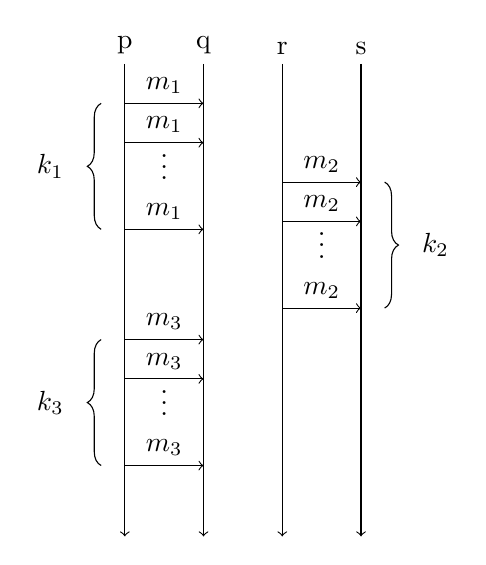
\begin{tikzpicture}
    \draw[->] (0,0) node [above] {p} -- (0,-6);
    \draw[->] (1,0) node [above] {q} -- (1,-6);
    \draw[->] (2,0) node [above] {r} -- (2,-6);
    \draw[->] (3,0) node [above] {s} -- (3,-6);

    \draw[->] (0,-.5) -- node [above] {$m_1$} (1,-.5);
    \draw[->] (0,-1) -- node [above] {$m_1$} (1,-1);
    \node at (.5,-1.2) {$\vdots$};
    \draw[->] (0,-2.1) -- node [above] {$m_1$} (1,-2.1);

    \draw[->] (2,-1.5) -- node [above] {$m_2$} (3,-1.5);
    \draw[->] (2,-2) -- node [above] {$m_2$} (3,-2);
    \node at (2.5,-2.2) {$\vdots$};
    \draw[->] (2,-3.1) -- node [above] {$m_2$} (3,-3.1);

    \draw[->] (0,-3.5) -- node [above] {$m_3$} (1,-3.5);
    \draw[->] (0,-4) -- node [above] {$m_3$} (1,-4);
    \node at (.5,-4.2) {$\vdots$};
    \draw[->] (0,-5.1) -- node [above] {$m_3$} (1,-5.1);

    % on ajoute des accolades
    \draw [decorate,decoration={brace,amplitude=5pt,mirror}] (-.3,-.5) -- node [midway, left=1em] {$k_1$} (-.3,-2.1) ;
    \draw [decorate,decoration={brace,amplitude=5pt,mirror}] (-.3,-3.5) -- node [midway, left=1em] {$k_3$} (-.3,-5.1) ;
    \draw [decorate,decoration={brace,amplitude=5pt}] (3.3,-1.5) -- node [midway, right=1em] {$k_2$} (3.3,-3.1) ;

\end{tikzpicture}

    \caption{The shape of the MSCs in $\msclanguageofcc{\gt_0}{}$ for the global type $\gt_0$.
    \label{fig:msc-regular}}
\end{figure} 

\begin{example}\label{ex:non-complementable-gt}
    Let $\Procs=\{p,q,r,s\}$, $\Messages=\{m_1,m_2,m_3\}$, and 
    $\Arrows=\{\gtlabel{p}{q}{m_1},\gtlabel{r}{s}{m_2},\gtlabel{p}{q}{m_3}\}$.
    First, consider a simple regular global type $\gt_0$ which MSCs linearisations 
    are of the form 
    $\{m_1^{k_1}m_2^{k_2}m_3^{k_3}\}$ (depicted in Fig.~\ref{fig:msc-regular}). 
    Note that $\gt_0$ is communitation-closed and
    $\existentialmsclanguageof{\gt_0}=\universalmsclanguageof{\gt_0}$.

    Second, consider the global type $\gt$ depicted in 
    Fig.~\ref{fig:non-complementable-gt-1}. 
    The linearisations of MSCs in $\existentialmsclanguageof{\gt}$ are 
    also of the form $\{m_1^{k_1}m_2^{k_2}m_3^{k_3}\}$ but 
    specifically with either $k_1\neq k_2$ or $k_2\neq k_3$.
    For instance, the upper branch of $\gt$ ensures that there is always at 
    least one $m_1$ more than $m_2$ in blue accepting states ($q_1$, $q_6$, $q_8$). 
    Similarly, the other branches ensure the other inequalities. 

    By contradiction suppose that  $\gt$ is complementable and  $\comp{\gt}$ is  its complement.
   Then $\gt''=\comp{\gt}\cap\gt_0$ exists and 
    since global type languages are closed under intersection with regular global types,
    $\gt''$ would still be a global type (in the form of a finite-state deterministic automaton).
    $\existentialmsclanguageof{\gt''}=\msclanguageofcc{\gt_0}{}\cap\existentialmsclanguageof{\gt'}$ 
    is the language of MSCs of the form %$\{m_1^{k_1}m_2^{k_2}m_3^{k_3}\}$ 
    %with $k_1=k_2=k_3$, i.e., all the MSCs of the form 
    $\{m_1^km_2^km_3^k\}$,  
    which no deterministic finite-state automaton, and therefore no global type, can recognise. 
    Thus, reaching a contradiction, hence $\gt''$, and $\comp{\gt}$ cannot exist, and $\gt$ is non-complementable.
\end{example}

\subsection{Effectively Complementable Global Types}

We say that complementation is effective for a class $\mathcal C$ of global types if 
there is a total, computable function $\gt \mapsto \comp{\gt}$ 
that takes as input a global type $\gt$ in $\mathcal C$ and computes its complement $\comp{\gt}$.

% \etienne{TODO changer les statements avec effective complementable.  
% Suggestions:
% - complementation is effective for a class of global types if 
% there is a procedure to effectively compute the complement of a given global type 
% in this class.
% - a class of global types is effectively complementable if there is a procedure to effectively compute the complement of a given global type in this class.
% }

\begin{proposition}\label{prop:commutation-closed-implies-complementable}
    Complementation is effective for the class of commutation-closed global types.
\end{proposition}

\begin{proof}
Let $\gt$ be a commutation-closed global type, and $Q,\delta$
be its  set of states and transition function. 
 $\comp{\gt}$ is the global type obtained by first completing 
$\gt$ (adding a sink state, so that the transition function $\delta:Q\times\Arrows\to Q$ is total),
and then swapping accepting and non-accepting states. 
Now, observe that 
$\existentialmsclanguageof{\comp{\gt}}=
\mscsetofmodel{\synchmodel}
\setminus \universalmsclanguageof{\gt}$. But, since $\gt$ is commutation closed:  
$\universalmsclanguageof{\gt}=\existentialmsclanguageof{\gt}$, concluding that 
$\comp{\gt}$ is a complement of $\gt$.
\end{proof}

As observed before, all global types with less than three participants are commutation closed, 
hence from Proposition~\ref{prop:commutation-closed-implies-complementable}
we have the following immediate result.

\begin{corollary}\label{coro:3-participants-complementable}
    Complementation is effective for the class of global types with $\cardinalof{\Procs}\leq 3$ participants.
\end{corollary}

More generally, we can show that all global types that are realisable in $\synchmodel$ 
are commutation-closed, and thus complementable.

\begin{theorem}\label{thm:realisable-complementable}
    Complementation is effective for the class of global types that are deadlock-free 
    realisable in $\synchmodel$.
\end{theorem}

\begin{proof}
    Let $\gt$ be a global type that is  deadlock-free realisable in $\synchmodel$.
    By condition~1 of Definition~\ref{def:realisability}, 
    $\executionsof{\projectionof{\gt}}{\synchmodel} = \executionsof{\gt}{\synchmodel}$.
    If two sets of executions are equal, the corresponding sets of their MSCs are also equal, 
    and thus $$\msclanguageof{\projectionof{\gt}}{\synchmodel}=\msclanguageof{\gt}{\synchmodel}.$$
    By construction, the synchronous product $\productof{\projectionof{\gt}}$
    is a global type whose runs are exactly the synchronous executions of the projected system, so 
    $$\msclanguageofcc{\productof{\projectionof{\gt}}}=\msclanguageof{\projectionof{\gt}}{\synchmodel}=\msclanguageof{\gt}{\synchmodel}.$$

    By Proposition~\ref{prop:product-is-commutation-closed}, $\productof{\projectionof{\gt}}$ is commutation-closed. 
    Thus, $\gt$ is also commutation-closed since they have the same MSCs language.
    Finally, by Proposition~\ref{prop:commutation-closed-implies-complementable},
    $\gt$ is complementable, and its proof  
    provides an effective algorithm for  complementation.
\end{proof}
    
\subsection{Sender-driven choice}

Stutz et al.  proved that $\ppmodel$-implementability (a notion close to realisability) 
is decidable for global types that satisfy sender-driven choice~\cite{DBLP:conf/cav/LiSWZ23}. We show that this can be seen as a consequence of the fact that global types with sender-driven choice are effectively complementable. We start by  recalling the definition of sender-driven choice.

\begin{definition}[Sender-driven choice]
    A global type $\gt$ has sender-driven choice
    if for all state $s$ of $\gt$, if $\gtlabel{p}{q}{m}$ and
    $\gtlabel{p'}{q'}{m'}$ label two transitions outgoing from $s$,
    then $p=p'$.
\end{definition}



\begin{figure*}[ht]
    \begin{tikzpicture}
        \begin{scope}
            \node at (-1,0) {$\gt~=$};
            \node[state,initial,initial text={},initial distance=3mm] (s0) at (1,0) {$s_0$};
            \node[state] (s1) at (3.5,1) {$s_1$};
            \node[state,accepting] (s2) at (7,0)  {$s_2$};
            \node[state,accepting] (s3) at (7,1) {$s_3$};
            \draw[->] (s0) -- node[above,sloped] {$\gtlabel{p}{q}{a_1}$} (s1);
            \draw[->] (s0) -- node[below,pos=0.15] {$\gtlabel{p}{q'}{a_2}$} (s2);
            \draw[->] (s1) -- node[above] {$\gtlabel{r}{r'}{b}$} (s3);
        \end{scope}
        \begin{scope}[xshift=8.5cm, yshift=1cm, scale=.5]
            \node at (0,0) {$M_1~=$};
            \draw[->] (1,1) node [above] {q}  -- (1,-1);
            \draw[->] (2,1) node [above] {p}  -- (2,-1);
            \draw[->] (3,1) node [above] {q'} -- (3,-1);
            \draw[->] (4,1) node [above] {r}  -- (4,-1);
            \draw[->] (5,1) node [above] {r'} -- (5,-1);
            \draw[->] (2,0) -- node [above] {$a_1$} (1,0);
            \draw[->] (4,0) -- node [above] {$b$} (5,0);
        \end{scope}
        \begin{scope}[xshift=8.5cm, yshift=-1cm, scale=.5]
            \node at (0,0) {$M_2~=$};
            \draw[->] (1,1) node [above] {q}  -- (1,-1);
            \draw[->] (2,1) node [above] {p}  -- (2,-1);
            \draw[->] (3,1) node [above] {q'} -- (3,-1);
            \draw[->] (4,1) node [above] {r}  -- (4,-1);
            \draw[->] (5,1) node [above] {r'} -- (5,-1);
            \draw[->] (2,0) -- node [above] {$a_2$} (3,0);
        \end{scope}
        \begin{scope}[yshift=-6cm]
            \node at (-1,0) {$\comp{\gt}~=$};
            \node[state,initial,initial text={},initial distance=3mm,accepting] (s0) at (1,0) {$s_0$};
            \node[state,accepting] (s1) at (3.5,2) {$s_1$};
            \node[state] (s2) at (6.5,0)  {$s_2$};
            \node[state] (s3) at (6.5,2) {$s_3$};
            \node[state,accepting] (s0b) at (6.5,-1.8) {$\comp{s_0}$};
            \node[state,accepting] (s1b) at (6.5,-4.2) {$\comp{s_1}$};
            \node[state,accepting] (sacc) at (11,2) {$s_{\mathsf{acc}}$};
            \node[state] (srej) at (11,-1.8) {$s_{\mathsf{rej}}$};
            \node[state,accepting] (sacc2) at (11,-4.2) {$s_{\mathsf{acc}}$};
            \draw[->] (s0) -- node[above,sloped] {$\gtlabel{p}{q}{a_1}$} (s1);
            \draw[->] (s0) -- node[above,sloped,pos=0.7] {$\gtlabel{p}{q'}{a_2}$} (s2);
            \draw[->] (s1) -- node[above,sloped] {$\gtlabel{r}{r'}{b}$} (s3);
            \draw[->] (s0) |- node[above,sloped,pos=.6] {$\gtlabel{(\neg p)}{(\neg p)}{\Messages}$} (s0b);
            \draw[->] (s1) |- node[above,sloped,pos=.7] {$\gtlabel{(\neg r)}{(\neg r)}{\Messages}$} (s1b);
            \draw[->,loop below] (s0b) edge node[below] {$\gtlabel{(\neg p)}{(\neg p)}{\Messages}$} ();
            \draw[->,loop below] (s1b) edge node[below] {$\gtlabel{(\neg r)}{(\neg r)}{\Messages}$} ();
            \draw[->,loop right] (sacc) edge node[right] {$\Arrows$} ();
            \draw[->,loop right] (srej) edge node[right] {$\Arrows$} ();
            \draw[->,loop right] (sacc2) edge node[right] {$\Arrows$} ();
            \draw[->] (s2) -- node[above,sloped] {$\Arrows$} (sacc);
            \draw[->] (s3) -- node[above,sloped] {$\Arrows$} (sacc);
            \draw[->] (s0b) -- node[above,sloped] {$\gtlabel{p}{q}{a_1}\vee\gtlabel{p}{q'}{a_2}$} (srej);
            \draw[->] (s1b) -- node[above,sloped] {$\gtlabel{r}{r'}{b}$} (srej);
            \draw[->] (s0b) -- node[above,sloped] {else} (sacc);
            \draw[->] (s1b) -- node[above,sloped] {else} (sacc2);
            \draw[->] (s1) edge[bend left] node[above,sloped,pos=.3] {else} (sacc);
            \draw[->] (s0) edge[bend left=60] node[above,sloped,pos=.2] {else} (sacc);

        \end{scope}

    \end{tikzpicture}
    \caption{A sender-driven global type $\gt$, with $\existentialmsclanguageof{\gt}=\{M_1,M_2\}$, and its
            complement $\comp{\gt}$ (for better readability, the state $s_{\mathsf{acc}}$ has been duplicated,
            the states $\comp{s_3}$ and $\comp{s_4}$, which are not reachable, have been omitted, and some transition labels have been summarized by Boolean expressions).
            \label{fig:example-of-sender-driven-gt-complementation}}
\end{figure*}


To prove that sender-driven global types are effectively complementable, we give the complementation procedure, and then show its correctness.
Let $\gt$ be a global type with sender-driven choice. 
For a sequence of arrows $w\in\Arrows^*$, 
 $\stateof{\gt,s}{w}$ is the state of $\gt$ reached after reading $w$ starting from
state $s$ (remember that $\gt$ is deterministic); note that $\stateof{\gt,s}{w}$ may be
undefined. For a state $s$ of $\gt$, let $\senderof{\gt}{s}$ be the process $p$
driving the choices in $s$, i.e., all outgoing transitions of $s$ are labeled with
arrows of the form $\gtlabel{p}{q}{m}$ for some $q,m$; note that $\senderof{\gt}{s}$
is undefined if $s$ has no outgoing transitions.

\begin{definition}[Complementation of a sender-driven global type]\label{def:complement-of-a-sender-driven-gt}
    Let $\gt$ be a sender-driven global type, and let $S$ be the set of states of $\gt$.
    Let $\comp{\gt}$ be the global type with set of states $S\cup\{\comp{s}\mid s\in S\}\cup\{s_{\mathsf{acc}},s_{\mathsf{rej}}\}$
    defined as follows:
    \begin{itemize}
        \item the initial state of $\comp{\gt}$ is the initial state of $\gt$;
        \item a state $s$ of $\gt$ is accepting in $\comp{\gt}$ if and only if 
        $s$ is non-accepting in $\gt$;
        \item for all state $s$ of $\gt$, $\comp{s}$ is accepting;
        \item $s_{\mathsf{acc}}$ is accepting, $s_{\mathsf{rej}}$ is non-accepting;
        \item for any two states $s,s'$ of $\gt$, $(s,\gtlabel{p}{q}{m},s')$ is a transition in $\comp{\gt}$ if and only if
        it is a transition in $\gt$;
        \item for any state $s$ of $\gt$, $(s,\gtlabel{p}{q}{m},\comp{s})$ (resp. $(\comp{s},\gtlabel{p}{q}{m},\comp{s})$) 
        is a transition in $\comp{\gt}$
        if and only if 
        \begin{itemize}
            \item $\gtlabel{p}{q}{m}$ is not labeling an outgoing transition of $s$,  
            \item $\senderof{\gt}{s}$ is defined, and
            \item $\senderof{\gt}{s}\not\in\{p,q\}$;
        \end{itemize}
        \item for any state $s$ of $\gt$, $(s,\gtlabel{p}{q}{m},s_{\mathsf{acc}})$  (resp. $(\comp{s},\gtlabel{p}{q'}{m},s_{\mathsf{acc}})$)
        is a transition in $\comp{\gt}$ 
        if and only if 
        \begin{itemize}
            \item $\gtlabel{p}{q}{m}$ is not labeling an outgoing transition of $s$ in $\gt$, and
            \item either $\senderof{\gt}{s}$ is undefined, or $\senderof{\gt}{s}\in\{p,q\}$,
        \end{itemize}
        \item for any state $s$ of $\gt$, $(\comp{s},\gtlabel{p}{q}{m},s_{\mathsf{rej}})$
        is a transition of $\comp{\gt}$ if and only if $\gtlabel{p}{q}{m}$ is labeling an outgoing transition of $s$ in $\gt$;
        \item $(s_{\mathsf{acc}},\gtlabel{p}{q}{m},s_{\mathsf{acc}})$ is a transition in $\comp{\gt}$ for all $p,q,m$;
        \item $(s_{\mathsf{rej}},\gtlabel{p}{q}{m},s_{\mathsf{rej}})$ is a transition in $\comp{\gt}$ for all $p,q,m$.
    \end{itemize}
\end{definition}


\begin{example}\label{ex:example-of-sender-driven-gt-complementation}
    Fig.~\ref{fig:example-of-sender-driven-gt-complementation} depicts a sender-driven global type
    and the complement computed according to Definition~\ref{def:complement-of-a-sender-driven-gt}.
\end{example}

It is easy to verify that $\comp{\gt}$ is deterministic, hence a global type. Note that $\comp{\gt}$
is also complete: for all $w\in\Arrows^*$, $\stateof{\comp{\gt}}{w}$ is defined. Moreover, 
the number of states of $\comp{\gt}$ is linear in the number of states of $\gt$, and that using Boolean
expressions to label transitions, the size of $\comp{\gt}$ can also be kept linear in the size of $\gt$.

\begin{theorem}\label{thm:sender-driven-choice-complementation}
    Complementation is effective for the class of global types with sender-driven choice.
\end{theorem}
%% PROOF in appendix


	\section{Decidability}\label{sec:decidability}
	
% !TEX root =  ../mainPPDP.tex
%!TEX spellcheck = en_GB

In this section, we show that the realisability problem for complementable global types,
given with an explicit complement, is decidable in both the synchronous and the p2p model.
We first show the result for the synchronous model, which is simpler,
and then extend it to the p2p model using a characterisation of implementability in the p2p model.

\subsection{Realisability in the synchronous model}

\begin{theorem}
    \label{thm:decidability-of-implementability-in-synch}
    Given a global type $\gt$ and its complement $\gt'$, it is decidable in PSPACE complexity whether  $\gt$ is deadlock-free realisable in $\synchmodel$.    
%  The  problem is in PSPACE:
  %  \begin{itemize}
    %    \item Input: a global type $\gt$ and a complement $\gt'$ of $\gt$.
      %  \item Question: is ?
    %\end{itemize}
\end{theorem}

\begin{proof}(Sketch)
    Condition~1 of Definition~\ref{def:realisability}
    is equivalent to $$\msclanguageofcc{\productof{\projectionof{\gt}}} \cap \existentialmsclanguageof{\gt'} = \emptyset,$$
    which reduces to checking the emptiness of $$\languageofnfa{\productof{\projectionof{\gt}}\otimes\gt'},$$
    where $\otimes$ is the standard product of NFAs mimicking intersection. This equivalence holds 
    because $\productof{\projectionof{\gt}}$ is commutation-closed. This condition
    can be checked in non-deterministic logarithmic space in the size of the product NFA,
    which yields a PSPACE algorithm if the exponential size NFA  $\preproductof{\projectionof{\gt}}$
    is lazily constructed (note that it is not necessary to determinise the NFA, as we only need to check emptiness). 
    Assuming that Condition~1 of Definition~\ref{def:realisability} holds,
    the second condition of Definition~\ref{def:realisability}  is 
    equivalent to whether all control states 
    of $\preproductof{\projectionof{\gt}}$ that are reachable from the initial state
    can reach a final state, which again can be checked in PSPACE.
\end{proof}

\subsection{Realisability in the $\ppmodel$ model}

%When moving to $\ppmodel$ the proof is significantly more involved and we need to resort  to  an equivalent  characterisation of deadlock-free realisability in the $\ppmodel$ model.

% !TEX root =  ../mainPPDP.tex
%!TEX spellcheck = en_GB

% \begin{lemma}\label{lem:synch-completion}
%     Assume $e$ is a synchronous execution, $\msc$ is a synchronous
%     MSC, and $\mscof{e}\prefixorder \msc$.
%     Then there is a synchronous execution $e'$ such that
%     $\msc=\mscof{e\cdot e'}$.
% \end{lemma}

% \begin{proof}
%     Let $e=s_0r_0s_1r_1..s_nr_n$ be a synchronous execution and 
%     $\msc$ is a synchronous MSC such that $\mscof{e}\prefixorder \msc$.
%     Let $e''=s''_0r''_0s''_1r''_1..s''_{n''}r''_{n''}$ be a synchronous linearization of $\msc$.
%     Since $\mscof{e}\prefixorder \msc$, we have that all events $s_i$ (and their respective $r_i$) 
%     of $e$ are present in $e''$. Let $e'$ be the restiction of $e''$ to the events that are not in $e$.
%     We get that $e'$ is a synchronous execution, and because $\mscof{e}\prefixorder \msc$, 
%     no event of $e$ is causally dependent on an event of $e'$ in $\msc$. Thus, 
%     $e'' \sim e\cdot e'$ and $\mscof{e\cdot e'}=\msc$.
% \end{proof}

\begin{theorem}\label{thm:pp-realizability-implies-synch-realizability}
    If $\gt$ is deadlock-free realisable in $\ppmodel$, then $\gt$ is deadlock-free realisable in $\synchmodel$.
\end{theorem}

\begin{proof}
Assume that $\gt$ is $\ppmodel$-realisable. We show that $\gt$ is $\synchmodel$-realisable by verifying the 
two conditions of Definition~\ref{def:realisability}.   
\begin{itemize}
\item 
    Since $\executionsofmodel{\synchmodel}\subseteq\executionsofmodel{\ppmodel}$, we have
    $$\mscsofcfsms{\projectionof{\gt}}{\synchmodel}\subseteq\mscsofcfsms{\projectionof{\gt}}{\ppmodel}.$$
    By Proposition~\ref{prop:msc-version-of-cond1-of-realizability} and the hypothesis that 
    $\gt$ is $\ppmodel$-realisable, we have that
    $$\mscsofcfsms{\projectionof{\gt}}{\ppmodel} \subseteq \existentialmsclanguageof{\gt}.
    $$
    Therefore, we have
    $$\mscsofcfsms{\projectionof{\gt}}{\synchmodel} \subseteq \existentialmsclanguageof{\gt}$$
    and by Proposition~\ref{prop:msc-version-of-cond1-of-realizability}, $\gt$ satisfies condition~1 of Definition~\ref{def:realisability}
    for being deadlock-free realisable in $\synchmodel$.

\item By Proposition~\ref{prop:deadlock-free-as-a-property-on-mscs-for-p2p-and-synch} and condition~1, the condition~2 of
    Definition~\ref{def:realisability} is equivalent to
    $$
        \mscsofcfsms{\projectionof{\acceptcompletion{\gt}}}{\acommunicationmodel}\subseteq\prefixclosureof{\existentialmsclanguageof{\gt}}
    $$
    when $\acommunicationmodel$ is either $\ppmodel$ or $\synchmodel$.
    We can therefore assume that 
    $$
        \mscsofcfsms{\projectionof{\acceptcompletion{\gt}}}{\ppmodel}\subseteq\prefixclosureof{\existentialmsclanguageof{\gt}}
    $$
    and we show that 
    $$
        \mscsofcfsms{\projectionof{\acceptcompletion{\gt}}}{\synchmodel}\subseteq\prefixclosureof{\existentialmsclanguageof{\gt}}
    $$
    This follows from the fact that
    $$
        \mscsofcfsms{\projectionof{\acceptcompletion{\gt}}}{\synchmodel}\subseteq\mscsofcfsms{\projectionof{\acceptcompletion{\gt}}}{\ppmodel}
    $$
    because $\executionsofmodel{\synchmodel}\subseteq\executionsofmodel{\ppmodel}$.
\end{itemize}
\end{proof}

%So we can state our main result.

\begin{restatable}[Reduction to $\synchmodel$-implementability]{theorem}{maintheoremrealisability}
    \label{thm:main-theorem-realisability}
        A global type $\gt$ is  deadlock-free realisable in $\ppmodel$
        if and only if the following four conditions hold:
        \begin{enumerate}
            \item $\msclanguageof{\projectionof{\gt}}{\ppmodel}\subseteq\prefixclosureof{\mscsetofmodel{\synchmodel}}$
            \item $\projectionof{\gt}$ is orphan-free in $\ppmodel$, 
            \item $\mscsofcfsms{\projectionof{\acceptcompletion{\gt}}}{\ppmodel}\subseteq\prefixclosureof{\mscsofcfsms{\projectionof{\gt}}{\ppmodel}}$, and 
            \item $\gt$ is deadlock-free realisable in $\synchmodel$.
        \end{enumerate}  
\end{restatable}
\begin{proof}
We show both sides in turn:
\begin{description}
    \item[$\Rightarrow$]
    We first show that the four conditions are necessary.
    Let $\gt$ be a $\ppmodel$-realisable global type.
    \begin{enumerate}
        \item        
            By Condition~2 of Definition~\ref{def:realisability},
            $\projectionof{\gt}$ is deadlock-free in $\ppmodel$.
            By Proposition~\ref{prop:deadlock-free-as-a-property-on-mscs-for-p2p-and-synch},
            $$
                \mscsofcfsms{\projectionof{\acceptcompletion{\gt}}}{\ppmodel}\subseteq\prefixclosureof{\mscsofcfsms{\projectionof{\gt}}{\ppmodel}}.
            $$
            By Condition~1 of Definition~\ref{def:realisability},
            $$
                \mscsofcfsms{\projectionof{\gt}}{\ppmodel} = \existentialmsclanguageof{\gt} \subseteq \mscsetofmodel{\synchmodel}.
            $$
            Therefore $\mscsofcfsms{\projectionof{\acceptcompletion{\gt}}}{\ppmodel}\subseteq\prefixclosureof{\mscsetofmodel{\synchmodel}}$.
   
        \item Let $e\in\executionsof{\projectionof{\gt}}{\ppmodel}$;
        we show that $e$ is orphan-free.
        By Condition~1 of Definition~\ref{def:realisability},
        $\mscof{e}\in\existentialmsclanguageof{\gt}$, therefore
        $\mscof{e}$ is synchronous, and in particular orphan-free.
       
        \item $\mscsofcfsms{\projectionof{\acceptcompletion{\gt}}}{\ppmodel}\subseteq\prefixclosureof{\mscsofcfsms{\projectionof{\gt}}{\ppmodel}}$ 
            by Condition~2 of Definition~\ref{def:realisability} and Proposition~\ref{prop:deadlock-free-as-a-property-on-mscs-for-p2p-and-synch}.

        \item  Follows from Lemma~\ref{thm:pp-realizability-implies-synch-realizability} 
    \end{enumerate}
\item[$\Leftarrow$]    Next we  show that the four conditions are sufficient.
    Let $\gt$ be a global type that verifies the four conditions.
%    \etienne{Ca marche pas! contre-exemple: $\gt = p->q:a + r->q:b$!}
    We prove that $\gt$ is $\ppmodel$-realisable as it satisfies the two conditions of Definition~\ref{def:realisability}.
    \begin{description}
        \item[Condition 1]
          By Proposition~\ref{prop:msc-version-of-cond1-of-realizability},
          we show that 
          $$
          \mscsofcfsms{\projectionof{\gt}}{\ppmodel} \subseteq \existentialmsclanguageof{\gt}.
          $$
          By Condition~1 of Theorem~\ref{thm:main-theorem-realisability},
          $$
            \mscsofcfsms{\projectionof{\gt}}{\ppmodel} = \mscsofcfsms{\projectionof{\gt}}{\synchmodel}
          $$
          and by Condition~4 of Theorem~\ref{thm:main-theorem-realisability} and Proposition~\ref{prop:msc-version-of-cond1-of-realizability},
          we have that  
          $$
            \mscsofcfsms{\projectionof{\gt}}{\synchmodel} \subseteq \existentialmsclanguageof{\gt}
          $$
          which concludes the proof of Condition~1.
          \item[Condition 2]
        follows from Proposition~\ref{prop:deadlock-free-as-a-property-on-mscs-for-p2p-and-synch}
        and Condition~3 of Theorem~\ref{thm:main-theorem-realisability}.
    \end{description}
\end{description}
\end{proof}
    
    
A system $\system$ such that 
$\msclanguageof{\system}{\ppmodel}\subseteq
\prefixclosureof{\mscsetofmodel{\synchmodel}}$
is called \emph{realisable with synchronous communications} (RSC) 
in~\cite{germerie-phd}. Germerie~\emph{et al.}~\cite{germerie-phd}
showed that the RSC property is decidable in PSPACE and that
whether a RSC system may reach a regular set of configurations is
also in PSPACE. As a consequence, conditions~1 and 2 of
Theorem~\ref{thm:main-theorem-realisability} can be checked in PSPACE.
Assuming that $\projectionof{\gt}$ is RSC, 
$\mscsofcfsms{\projectionof{\acceptcompletion{\gt}}}{\ppmodel}$ can be coded as an effective regular set of
executions, as well as $\prefixclosureof{\mscsofcfsms{\projectionof}{\ppmodel}}$,
and Condition~3 of Theorem~\ref{thm:main-theorem-realisability} reduces to checking the inclusion of
two exponential size NFA, which can be checked in PSPACE using a lazy construction of the NFAs.


% It remains to show that the third condition of
% Theorem~\ref{thm:main-theorem-implementability}
% is decidable in PSPACE. 
% This relies on the following lemma that states that 
% condition~3 of Theorem~\ref{thm:main-theorem-realisability} is equivalent to
% being dead-lock free in the sense of Definition~\ref{def:orphan-deadlock-free}.

% \begin{restatable}{lemma}{eventualterminationonmsc}\label{lem:eventual-termination-can-be-checked-on-mscs-for-p2p}
%     $\executionsof{\projectionof{\acceptcompletion{\gt}}}{\ppmodel}=\prefixclosureof{\executionsof{\projectionof{\gt}}{\ppmodel}}$ is equivalent to
%     is equivalent to $\gt$ being deadlock-free in $\ppmodel$.
% \end{restatable}
% \begin{proof}
    Let $\cfsms=\projectionof{\gt}$.
    \begin{description}
        \item[$\Rightarrow$]
            Let $e\in\executionsofcfsms{\acceptcompletion{\cfsms}}{\acommunicationmodel}\setminus \executionsofcfsms{\cfsms}{\acommunicationmodel}$.
            By the left-hand equality, $e$ is a strict prefix of some
            $e' \in \executionsofcfsms{\cfsms}{\acommunicationmodel} \subseteq \executionsofcfsms{\acceptcompletion{\cfsms}}{\acommunicationmodel}$;
            hence $\cfsms$ can extend $e$, so the reached configuration is not a dead-lock.
        \item[$\Leftarrow$]
            First inclusion is trivial because every word of $\executionsofcfsms{\cfsms}{\acommunicationmodel}$ is accepted by $\cfsms$.
            For the reverse inclusion, let $e\in\executionsofcfsms{\acceptcompletion{\cfsms}}{\acommunicationmodel}$
            If $e\in \executionsofcfsms{\cfsms}{\acommunicationmodel}$ we are done; otherwise deadlock freedom supplies an extension $e'$ of $e$ that is in
             $\executionsofcfsms{\acceptcompletion{\cfsms}}{\acommunicationmodel}$; iterate until a configuration of $\cfsms$ in which all peers are final is met. 
            The concatenation of the successive extensions belongs to $\executionsofcfsms{\cfsms}{\acommunicationmodel}$ and has $e$ as prefix.
    \end{description}
\end{proof}

From these results we can conclude that it can be decided in PSPACE that a given $\gt$,
together with a complement hint, is deadlock-free realisable in the $\ppmodel$ model.
 \begin{theorem}\label{thm:decidability-of-implementability-in-p2p}
   
   Given a complementable global type $\gt$ and its complement $\gt'$,     it is decidable in PSPACE complexity whether $\gt$ is deadlock-free realisable in $\ppmodel$.
   
%       The following problem is in PSPACE:
 %\begin{itemize}
  %      \item Input: a complementable global type $\gt$ and a complement $\gt'$ of $\gt$.
    %    \item Question: is $\gt$ deadlock-free realisable in $\ppmodel$?
    %\end{itemize}
\end{theorem}



	\section{Concluding remarks} \label{sec:concl}	
	  % !TEX root =  ../mainPPDP.tex
%!TEX spellcheck = en_GB

In this paper, we investigated the realisability and complementability of MPSTs across two canonical communication models: synchronous and asynchronous ($\ppmodel$). 
We reduce the task of checking realisability in the complex asynchronous setting to the simpler synchronous case, as long as the initial system satisfies key safety properties such as deadlock-freedom and absence of orphan messages.
This reduction strongly depends on the notion of effective complementability. 
Our results show that existing work -— such as sender-driven global types~\cite{DBLP:conf/cav/LiSWZ23} and protocols with at most three participants -— belongs to effectively complementable classes of global types and thus confirms the decidability thresholds that Alur et al.~\cite{DBLP:journals/tcs/AlurEY05} and Lohrey~\cite{DBLP:journals/tcs/Lohrey03} established.

We believe that our results not only improve theoretical clarity but also are amenable to generalisation. This paper represents a first step towards a parametric framework for realisability checking, with potential applicability across diverse communication models. Throughout the paper, we have made a deliberate effort to explicitly state the hypotheses (related to the communication model) under which our theorems hold. 
A particularly critical assumption is that the communication models in question must be causally closed (see Definition \ref{def:causally-closed-communication-model}). Based on this, we conjecture that our results can be extended to models such as bag and causally ordered systems, both of which satisfy causal closure. In contrast, models like mailbox  or those based on bounded FIFO channels lack this property and therefore require specialised analysis. We aim to explore these cases further and, ultimately, to develop a more comprehensive framework in future work.

Apart from this generalisation,  we aim to extend the framework to cover more expressive classes of global types, including those that go beyond synchronous or (quasi-synchronous) behaviour. We also plan to revisit results on the realisability of MSCs, possibly linking criteria such as send-validity and receive-validity \cite{DBLP:conf/cav/LiSWZ23,DBLP:conf/ecoop/Stutz23} to our synchronous realisability conditions. This opens the door to formally investigating whether global types that are realisable in the synchronous model satisfy send-validity, or if this is a weaker or stronger condition—this remains an open and promising question.


Our work brings that line of research into the realm of programming language design with MPST: we build upon the insights of MSC realisability (e.g., the importance of safety conditions for realisability) and apply them in a type-theoretic framework to obtain results directly applicable to real programming abstractions for concurrency. 
In summary, by focusing on $\ppmodel$ and synchronous communication models, we shed new light on the implementability of multiparty protocols in practical distributed programming, overcoming the limitations of sender-driven choice and advancing the state of the art in MPST-based program verification.

\subsubsection*{\bf Related works}
We conclude with a brief excursus on related work. Naturally, the most closely related lines of research are those concerning MPST. Comprehensive surveys on the topic are available in \cite{Coppo2015, DBLP:conf/icdcit/YoshidaG20}.
It is noteworthy that in standard MPST literature, realisability—often referred to as implementability—is typically addressed through syntactic restrictions on global types. In most cases, a global type is  implementable if a projection function exists. These syntactic constraints, along with the existence of the projection, imply that the global type is sender-driven, thus placing it within one of the complementable classes discussed in this paper.
In contrast, a recent paper by Scalas and Yoshida~\cite{DBLP:journals/pacmpl/ScalasY19} offers a novel perspective. Their approach emphasizes session fidelity and deliberately abandons syntactic restrictions on session types. Instead, they adopt semantic criteria—validated through model checking—to establish implementability, marking a significant shift from the conventional syntactic paradigm or our approach.
Although, the comparison is difficult as the underliniung models are substantially different, it is wort mentioning \cite{10.1145/3678232.3678245} that discusses projectability in the context of synchronous MPST. 



The connection between communicating automata and behavioural types were 
first explored by Villard \cite{villard-phd} for the binary case and Deniélou and Yoshida in \cite{DBLP:conf/esop/DenielouY12} for MPSTs and later exploited by Stutz \emph{et al.} in \cite{DBLP:conf/cav/LiSWZ23,DBLP:conf/ecoop/Stutz23}.
Although our approach automata-theoretic approach of session types is not new, it is 
perphaps not so well established, and most of the papers on MPST define them syntactically.
We took a fundamentally semantic view of session types, considering them as the subclass of higher order message sequence charts 
that specify only protocols that are realisable with synchronous communications. This point of view is highly debatable, but 
helps to clarify the relation between MPST and HMSCs.


In~\cite{DBLP:conf/cav/LiSWZ23,DBLP:conf/ecoop/Stutz23}, the authors revisited
the theory of MPST projections through the lenses of realisability
of MSCs, and proposed two criteria, called \emph{send validity} and {receive validity},
that yield the first sound and complete
characterisation of MPST implementable in the context of
the $\ppmodel$ communication model, provided the global type is sender-driven.
In particular, the second criteria, receive validity,
is strongly justified by the choice of the communication model and is unsound for
other communication models beyond $\ppmodel$, hence not generalisable. As already commented above %
%Finally, we contrast our approach with existing work. 
%Stutz et al.~\cite{DBLP:conf/cav/LiSWZ23} investigate asynchronous MPST implementability using an automata-theoretic approach, constructing communicating automata to represent protocol executions. 
 our approach provides a semantic criterion for implementability that leverages a reduction to the synchronous case, and it identifies a wider decidable subclass of global types (effectively complementable protocols) that covers the class of systems considered by Stutz et al. as a special case. 
 
On a more foundational level, global types can be seen as a special form of higher-order message sequence charts (HMCS, see~\cite{DBLP:journals/tcs/AlurEY05}) with synchronous communications. 
Thus, the question of when a global specification is realisable by a distributed system is related to the classical MSC realisability problem studied by Alur et al. In particular, the implementability problem was formally introduced by Alur et al. \cite{DBLP:journals/tcs/AlurEY05} with early undecidability results, later simplified by Lohrey \cite{DBLP:journals/tcs/Lohrey03}. Our results refine these boundaries by showing that undecidability persists with four or more participants.
Guanciale and Tuosto \cite{DBLP:journals/jlap/GuancialeT19} extended these results on pomsets, we plan to build on their work to generalise to other communication models.


%As a matter of fact, most of the MPST theory focuses on the peer-to-peer communication model only. To the best of our knowledge, the few attempts in considering other communicating models for MPST 
%only concern mailbox communications~\cite{DBLP:journals/pacmpl/FowlerASGT23,deliguoro_et_al:LIPIcs.ECOOP.2018.15}.

%The second group of related works concerns the framework of implementability. In particular, QS systems are a generalisation of RSC systems as introduced in \cite{DBLP:journals/corr/abs-2110-00145}. The notion of "synchronizable"
%communications can also be found as a special case in other works,
%including existentially-bounded communications~\cite{DBLP:journals/fuin/GenestKM07} or $1$-synchronous communications~\cite{DBLP:conf/cav/BouajjaniEJQ18}. 
%
%Finally, although less related to the content of this paper, we want to point to discussions and relations among communication models:  \cite{DBLP:journals/dc/Charron-BostMT96,ENGELS2002253,DBLP:conf/fm/ChevrouH0Q19} and \cite{DBLP:journals/pacmpl/GiustoFLL23}.



%\etienne{A rediscuter avec Cinzia. Il faudrait que chaque papier soit relie precisement à notre travail sur une de nos contributions. Ou alors on a aussi un section related work d'un point de vue "historique", sans forcement de lien plus profond avec notre travail, mais il faudrait distinguer les deux types de related works, historiques, et concurrentiels/complementaires.}




%\etienne{Pour moi l'un des "breakthrough" de Stutz c'est davoir defini la projection de maniere inconditionnelle, meme pour les global types non implementable. C'est trivial mais la communaute session types ne l'avait pas fait avant, il me semble}
%\cinzia{Je ne comprends pas ce que tu veux dire}

%\etienne{Il faudrait dire que l'on aimerait relier ces deux critères à nos resultats, en particulier send validity qui semble assez fondamental: est-ce que l'on peut dire que les global types implementables en synchrone sont ceux qui satisfont send validity? condition plus faible? plus forte?}




%\etienne{Citer Baudru-Morin pour l'implementabilite en bag.}


%\etienne{Dans les personnes "trendy" a ne pas oublier: citer Bouajjani Enea pour leur papier CAV'07 qui introduit la technique de borderline violation. Citer aussi Azadeh Farzan, par exemple LICS'2023, sur les langages de mots avec des lettres qui commutent (a creuser)}

%\cinzia{A part le dernier, ce 'est plus applicable }


%A CITER \cite{DBLP:conf/snpd/BaudruM03}.

%A CITER: un vieux papier avec Jules sur les binary session types (appelés communication contracts)
%interprétés dans des modèles de communication non fiables (avec des pertes de messages, des duplications, etc.).
%\cite{DBLP:conf/wsfm/LozesV11}.








%%
%% The acknowledgments section is defined using the "acks" environment
%% (and NOT an unnumbered section). This ensures the proper
%% identification of the section in the article metadata, and the
%% consistent spelling of the heading.
% \begin{acks}
% To Robert, for the bagels and explaining CMYK and color spaces.
% \end{acks}

%%
%% The next two lines define the bibliography style to be used, and
%% the bibliography file.
\bibliographystyle{ACM-Reference-Format}
\bibliography{refs}


%%
%% If your work has an appendix, this is the place to put it.
%\iflong
%\else
%\appendix
%% !TEX root =  ../mainPPDP.tex
%!TEX spellcheck = en_GB

%\section{Proof of Lemma~\ref{lem:pp-is-causally-closed}}
%\label{app:pp-is-causally-closed}

%% !TEX root =  ../mainPPDP.tex
%!TEX spellcheck = en_GB
Observe that not all communication models are causally closed. It is the case for $\ppmodel$,  but it is immediate  to see that the property is not valid  for $\synchmodel$. Take for instance  MSC $M$ in Fig.~\ref{fig:rsc_ex},  its linearisation 
$!m_1!m_2?m_1?m_2!m_3?m_3$ 
  does not belong to $\linearisationsof{M_c}{\synchmodel}$.  To show that $\ppmodel$ is causally closed, 
notice that $<$ can be replaced with $\porderof{M}$ in  Definition~\ref{def:queue-based-communication-model}.
\begin{lemma}\label{lem:reformulation-of-ppmodel-def}
    Let $e$ be an execution and  $M=\mscof{e}$.
    Then $e$ is an execution of $\ppmodel$ if and only if
    for any two send events $s_1=\send{p}{q}{\msg_1}$ and $s_2=\send{p}{q}{\msg_2}$ in $\sendeventsof{e}$, with $s_1 \porderof{M} s_2$,
        one of the two holds:
        \begin{itemize}
            \item $s_2$ is unmatched, or
            \item there exists $r_1,r_2$ such that $r_1 \porderof{M} r_2$, $\source(r_1)=s_1$, and $\source(r_2)=s_2$.
        \end{itemize}
\end{lemma}
\begin{proof}
    Assume that $e$ is a $\ppmodel$ execution.
    Let $s_1=\send{p}{q}{\msg_1}$ and $s_2=\send{p}{q}{\msg_2}$ be two send events in $\sendeventsof{e}$ such that $s_1 \porderof{M} s_2$.
    Then $s_1<s_2$ in $e$, because $<$ is a linearisation of $\porderof{M}$.
    By  definition of $\ppmodel$, $s_2$ is unmatched or there exists $r_1,r_2$ such that $r_1 < r_2$, $\source(r_1)=s_1$, and $\source(r_2)=s_2$.
    In the second case, $r_1 < r_2$ implies that
    $r_1 \porderof{M} r_2$, because both $r_1$ and $r_2$ occur on the same process $q$.
    Conversely, assume that $e$ and $M$ satisfy the above reformulation of the definition of $\ppmodel$. 
    Let $s_1=\send{p}{q}{\msg_1}$ and $s_2=\send{p}{q}{\msg_2}$ be two send events in $\sendeventsof{e}$ such that $s_1 < s_2$.
    Then $s_1 \porderof{M} s_2$
    because $s_1$ and $s_2$ occur on the same process $p$.
    By the reformulation of the definition of $\ppmodel$, $s_2$ is unmatched or there exists $r_1,r_2$ such that $r_1 \porderof{M} r_2$, $\source(r_1)=s_1$, and $\source(r_2)=s_2$.
    In the second case, $r_1 \porderof{M} r_2$
    implies that $r_1 < r_2$ because $<$ is a  linearisation of $\porderof{M}$.
\end{proof}

\begin{restatable}[]{lemma}{lemppiscasuallyclosed}\label{lem:pp-is-causally-closed}
	$\executionsofmodel{\ppmodel}$ is causally-closed.
\end{restatable}
\begin{proof}
    Let $M\in\mscsetofmodel{\ppmodel}$ 
    and  $e$ be a linearisation of $M$.
    We want to show that $e\in\executionsofmodel{\ppmodel}$.
    By definition of $\mscsetofmodel{\ppmodel}$, 
    there is an execution 
    $e'\in\executionsofmodel{\ppmodel}$
    such that $\mscof{e'}=M$.
    By Lemma~\ref{lem:reformulation-of-ppmodel-def},
    $e$ is also a $\ppmodel$ execution.
\end{proof}

%\section{Proof of Proposition~\ref{prop:deadlock-free-as-a-property-on-mscs-for-p2p-and-synch}}
%\label{app:deadlock-free-as-a-property-on-mscs-for-p2p-and-synch}

%\propdeadlockfreeasapropertyonmscsforppandsynch*
%% !TEX root =  ../mainPPDP.tex
%!TEX spellcheck = en_GB

\begin{proof}
    We show each implication separately.
    \begin{description}
        \item[$\Rightarrow$:]
        if $\cfsms$ is deadlock-free: $\executionsof{\acceptcompletion{\cfsms}}{\acommunicationmodel}\subseteq\prefixclosureof{\executionsof{\cfsms}{\acommunicationmodel}}$, 
        then 
        $\msclanguageof{\acceptcompletion{\cfsms}}{\acommunicationmodel}\subseteq
        \prefixclosureof{\msclanguageof{\cfsms}{\acommunicationmodel}}$.
        For this implication, $\acommunicationmodel$ can be any communication model.
        Let $\msc\in\msclanguageof{\acceptcompletion{\cfsms}}{\acommunicationmodel}$, 
       we show that $\msc\in\prefixclosureof{\msclanguageof{\cfsms}{\acommunicationmodel}}$.
        By definition, there is an execution $e\in\executionsof{\acceptcompletion{\cfsms}}{\acommunicationmodel}$ such that $\msc=\mscof{e}$.
        By hypothesis, there is a completion $e' \in\executionsof{\cfsms}{\acommunicationmodel}$ of $e$.
        By definition, $\mscof{e'}\in\msclanguageof{\acceptcompletion{\cfsms}}{\acommunicationmodel}$,
        so $\msc\in\prefixclosureof{\msclanguageof{\cfsms}{\acommunicationmodel}}$.

        \item[$\Leftarrow$:] for  $\acommunicationmodel=\ppmodel$:
        if  
        $\msclanguageof{\acceptcompletion{\cfsms}}{\acommunicationmodel}\subseteq
        \prefixclosureof{\msclanguageof{\cfsms}{\acommunicationmodel}}$,
        then $\cfsms$ is deadlock-free.
        Let $e\in\executionsof{\acceptcompletion{\cfsms}}{\acommunicationmodel}$ be an execution,
        wez show that $e$ has a completion in $\executionsof{\cfsms}{\acommunicationmodel}$.
        By definition, $\mscof{e}\in\msclanguageof{\acceptcompletion{\cfsms}}{\acommunicationmodel}$.
        By hypothesis, there is a MSC $\msc'\in\msclanguageof{\cfsms}{\acommunicationmodel}$
        such that $\mscof{e}\prefixordermsc\msc'$. By definition of $\prefixordermsc$ on MSCs,
        there are two executions $e_1,e'$ such that 
        $e_1\prefixorder e'$, $\mscof{e'}=\msc'$, 
        and $\mscof{e_1}=\mscof{e}$.
        Let $<$ be the binary relation on $\eventsof{M'}$ 
        defined as $< \eqdef \torderstrictof{e}\cup <_1\cup <_2$, where:
        \begin{itemize}
            \item $\event <_1<\event'$ if $\event\not\in\eventsof{M}$,
            $\event'\not\in\eventsof{M}$ and $\event <_{e'} \event'$;
            \item $\event <_2\event'$ if $\event\in\eventsof{M}$ and $\event'\not\in\eventsof{M}$.
        \end{itemize}
        Note that $<_1$ and $<_2$ are transitive. We claim that $<$
        is also transitive. Indeed, 
        $$
        \begin{array}{rcl}
           \torderof{e}\cdot <_1 & = & <_1\\
            <_1\cdot <_2 & = & <_1 \\
            \torderof{e}\cdot<_2 & = & \emptyset \\
            (<_1\cup <_2)\cdot \torderof{e} & = & \emptyset \\
            (\torderof{e}\cup <_2)\cdot <_1 & = & \emptyset \\
        \end{array}
        $$
        Moreover, $<$ is irreflexive, because $\torderof{e}$ is irreflexive and $<_1$ and $<_2$ are irreflexive.
        Let $\leq$ denote the reflexive closure of $<$.
        Then this is a partial order on $\eventsof{M'}$.
        By construction, $\leq$ is actually a total order on $\eventsof{M'}$.       
        Finally, we claim that $\leq$ is a linearisation of $M'$, i.e., $\porderof{M'}\subseteq \leq$.
        Indeed, assume that $\event\porderstrictof{M'}\event'$, we show that $\event< \event'$:
        \begin{itemize}
            \item if $\event\in\eventsof{M}$ and $\event'\in\eventsof{M}$,
            then $\event\porderstrictof{M} \event'$ (as $M$ is a prefix of $M'$), hence $\event\torderof{e} \event'$ 
            (because $e$ is a linearisation of $M$),
            and finally $\event < \event'$ by definition of $<$.
            
            \item if $\event\not\in\eventsof{M}$ and $\event'\not\in\eventsof{M}$,
            then $\event\torderof{e'} \event'$ (because $e'$ is a linearisation of $M'$), 
            therefore $\event <_1 \event'$ by definition of $<_1$, and finally $\event < \event'$ by definition of $<$.

            \item if $\event\in\eventsof{M}$ and $\event'\not\in\eventsof{M'}$,
            then $\event<_2 \event'$ by definition of $<_2$, therefore $\event < \event'$ by definition of $<$.
        \end{itemize}
        Therefore, $\leq$ is a linearisation of $M'$. Let $e''$ be the execution associated to $\leq$.
        Then
        \begin{itemize}
            \item $e\prefixorder e''$ by definition of $\leq$;
            \item $\mscof{e''}=M'$ as $\leq$ is a linearisation of $M'$;
            \item $e''\in\executionsof{\cfsms}{\acommunicationmodel}$ because $e''$ is a linearisation of $M'$, $M'\in\msclanguageof{\cfsms}{\acommunicationmodel}$,
            and $\ppmodel$ is causally closed (Lemma~\ref{lem:pp-is-causally-closed}).
        \end{itemize}
        Altogether, we have shown that $e$ has a completion in $\executionsof{\cfsms}{\acommunicationmodel}$, which ends the proof of 
        the reverse implication.

        \item[$\Leftarrow$:]   for $\acommunicationmodel=\synchmodel$:
            the proof is similar to previous case. We define the linearisation $\leq$ of $M'$ 
            in the exactly  same way, but we cannot use the fact that $\acommunicationmodel$ is causally closed.
            Instead, we use the fact that both $<_e$ and  $<_1$ are synchronous linearisations,
            and therefore $<$ is a synchronous linearisation as the concatenation of two synchronous linearisations.

    \end{description}
\end{proof}

%\section{Proof of Theorem~\ref{thm:main-theorem-realisability}}
%\label{app:main-theorem-realisability}
%\maintheoremrealisability*
%% !TEX root =  ../mainPPDP.tex
%!TEX spellcheck = en_GB

% \begin{lemma}\label{lem:synch-completion}
%     Assume $e$ is a synchronous execution, $\msc$ is a synchronous
%     MSC, and $\mscof{e}\prefixorder \msc$.
%     Then there is a synchronous execution $e'$ such that
%     $\msc=\mscof{e\cdot e'}$.
% \end{lemma}

% \begin{proof}
%     Let $e=s_0r_0s_1r_1..s_nr_n$ be a synchronous execution and 
%     $\msc$ is a synchronous MSC such that $\mscof{e}\prefixorder \msc$.
%     Let $e''=s''_0r''_0s''_1r''_1..s''_{n''}r''_{n''}$ be a synchronous linearization of $\msc$.
%     Since $\mscof{e}\prefixorder \msc$, we have that all events $s_i$ (and their respective $r_i$) 
%     of $e$ are present in $e''$. Let $e'$ be the restiction of $e''$ to the events that are not in $e$.
%     We get that $e'$ is a synchronous execution, and because $\mscof{e}\prefixorder \msc$, 
%     no event of $e$ is causally dependent on an event of $e'$ in $\msc$. Thus, 
%     $e'' \sim e\cdot e'$ and $\mscof{e\cdot e'}=\msc$.
% \end{proof}

\begin{theorem}\label{thm:pp-realizability-implies-synch-realizability}
    If $\gt$ is deadlock-free realisable in $\ppmodel$, then $\gt$ is deadlock-free realisable in $\synchmodel$.
\end{theorem}

\begin{proof}
Assume that $\gt$ is $\ppmodel$-realisable. We show that $\gt$ is $\synchmodel$-realisable by verifying the 
two conditions of Definition~\ref{def:realisability}.   
\begin{itemize}
\item 
    Since $\executionsofmodel{\synchmodel}\subseteq\executionsofmodel{\ppmodel}$, we have
    $$\mscsofcfsms{\projectionof{\gt}}{\synchmodel}\subseteq\mscsofcfsms{\projectionof{\gt}}{\ppmodel}.$$
    By Proposition~\ref{prop:msc-version-of-cond1-of-realizability} and the hypothesis that 
    $\gt$ is $\ppmodel$-realisable, we have that
    $$\mscsofcfsms{\projectionof{\gt}}{\ppmodel} \subseteq \existentialmsclanguageof{\gt}.
    $$
    Therefore, we have
    $$\mscsofcfsms{\projectionof{\gt}}{\synchmodel} \subseteq \existentialmsclanguageof{\gt}$$
    and by Proposition~\ref{prop:msc-version-of-cond1-of-realizability}, $\gt$ satisfies condition~1 of Definition~\ref{def:realisability}
    for being deadlock-free realisable in $\synchmodel$.

\item By Proposition~\ref{prop:deadlock-free-as-a-property-on-mscs-for-p2p-and-synch} and condition~1, the condition~2 of
    Definition~\ref{def:realisability} is equivalent to
    $$
        \mscsofcfsms{\projectionof{\acceptcompletion{\gt}}}{\acommunicationmodel}\subseteq\prefixclosureof{\existentialmsclanguageof{\gt}}
    $$
    when $\acommunicationmodel$ is either $\ppmodel$ or $\synchmodel$.
    We can therefore assume that 
    $$
        \mscsofcfsms{\projectionof{\acceptcompletion{\gt}}}{\ppmodel}\subseteq\prefixclosureof{\existentialmsclanguageof{\gt}}
    $$
    and we show that 
    $$
        \mscsofcfsms{\projectionof{\acceptcompletion{\gt}}}{\synchmodel}\subseteq\prefixclosureof{\existentialmsclanguageof{\gt}}
    $$
    This follows from the fact that
    $$
        \mscsofcfsms{\projectionof{\acceptcompletion{\gt}}}{\synchmodel}\subseteq\mscsofcfsms{\projectionof{\acceptcompletion{\gt}}}{\ppmodel}
    $$
    because $\executionsofmodel{\synchmodel}\subseteq\executionsofmodel{\ppmodel}$.
\end{itemize}
\end{proof}

%So we can state our main result.

\begin{restatable}[Reduction to $\synchmodel$-implementability]{theorem}{maintheoremrealisability}
    \label{thm:main-theorem-realisability}
        A global type $\gt$ is  deadlock-free realisable in $\ppmodel$
        if and only if the following four conditions hold:
        \begin{enumerate}
            \item $\msclanguageof{\projectionof{\gt}}{\ppmodel}\subseteq\prefixclosureof{\mscsetofmodel{\synchmodel}}$
            \item $\projectionof{\gt}$ is orphan-free in $\ppmodel$, 
            \item $\mscsofcfsms{\projectionof{\acceptcompletion{\gt}}}{\ppmodel}\subseteq\prefixclosureof{\mscsofcfsms{\projectionof{\gt}}{\ppmodel}}$, and 
            \item $\gt$ is deadlock-free realisable in $\synchmodel$.
        \end{enumerate}  
\end{restatable}
\begin{proof}
We show both sides in turn:
\begin{description}
    \item[$\Rightarrow$]
    We first show that the four conditions are necessary.
    Let $\gt$ be a $\ppmodel$-realisable global type.
    \begin{enumerate}
        \item        
            By Condition~2 of Definition~\ref{def:realisability},
            $\projectionof{\gt}$ is deadlock-free in $\ppmodel$.
            By Proposition~\ref{prop:deadlock-free-as-a-property-on-mscs-for-p2p-and-synch},
            $$
                \mscsofcfsms{\projectionof{\acceptcompletion{\gt}}}{\ppmodel}\subseteq\prefixclosureof{\mscsofcfsms{\projectionof{\gt}}{\ppmodel}}.
            $$
            By Condition~1 of Definition~\ref{def:realisability},
            $$
                \mscsofcfsms{\projectionof{\gt}}{\ppmodel} = \existentialmsclanguageof{\gt} \subseteq \mscsetofmodel{\synchmodel}.
            $$
            Therefore $\mscsofcfsms{\projectionof{\acceptcompletion{\gt}}}{\ppmodel}\subseteq\prefixclosureof{\mscsetofmodel{\synchmodel}}$.
   
        \item Let $e\in\executionsof{\projectionof{\gt}}{\ppmodel}$;
        we show that $e$ is orphan-free.
        By Condition~1 of Definition~\ref{def:realisability},
        $\mscof{e}\in\existentialmsclanguageof{\gt}$, therefore
        $\mscof{e}$ is synchronous, and in particular orphan-free.
       
        \item $\mscsofcfsms{\projectionof{\acceptcompletion{\gt}}}{\ppmodel}\subseteq\prefixclosureof{\mscsofcfsms{\projectionof{\gt}}{\ppmodel}}$ 
            by Condition~2 of Definition~\ref{def:realisability} and Proposition~\ref{prop:deadlock-free-as-a-property-on-mscs-for-p2p-and-synch}.

        \item  Follows from Lemma~\ref{thm:pp-realizability-implies-synch-realizability} 
    \end{enumerate}
\item[$\Leftarrow$]    Next we  show that the four conditions are sufficient.
    Let $\gt$ be a global type that verifies the four conditions.
%    \etienne{Ca marche pas! contre-exemple: $\gt = p->q:a + r->q:b$!}
    We prove that $\gt$ is $\ppmodel$-realisable as it satisfies the two conditions of Definition~\ref{def:realisability}.
    \begin{description}
        \item[Condition 1]
          By Proposition~\ref{prop:msc-version-of-cond1-of-realizability},
          we show that 
          $$
          \mscsofcfsms{\projectionof{\gt}}{\ppmodel} \subseteq \existentialmsclanguageof{\gt}.
          $$
          By Condition~1 of Theorem~\ref{thm:main-theorem-realisability},
          $$
            \mscsofcfsms{\projectionof{\gt}}{\ppmodel} = \mscsofcfsms{\projectionof{\gt}}{\synchmodel}
          $$
          and by Condition~4 of Theorem~\ref{thm:main-theorem-realisability} and Proposition~\ref{prop:msc-version-of-cond1-of-realizability},
          we have that  
          $$
            \mscsofcfsms{\projectionof{\gt}}{\synchmodel} \subseteq \existentialmsclanguageof{\gt}
          $$
          which concludes the proof of Condition~1.
          \item[Condition 2]
        follows from Proposition~\ref{prop:deadlock-free-as-a-property-on-mscs-for-p2p-and-synch}
        and Condition~3 of Theorem~\ref{thm:main-theorem-realisability}.
    \end{description}
\end{description}
\end{proof}


\section{Discussion about deadlock-free realizability and safe realizability}
\label{app:discussion-deadlock-free-realizability-and-safe-realizability}
\etienne{TODO: retrouver les éléments de la discussion dans les versions antérieures ou dans la réponse au reviewer}
%\fi

\end{document}
\endinput
%%
%% End of file `sample-sigplan.tex'.
